\documentclass{article}
\usepackage{filecontents}
\usepackage[left=2.5cm,top=2.5cm,right=2.5cm,bottom=2.5cm]{geometry}
\usepackage{amsmath}
\usepackage{array}
\usepackage{caption}
\usepackage{placeins}
\usepackage[colorlinks=true,citecolor=blue]{hyperref}
\usepackage{graphicx}
\usepackage{subcaption}
\usepackage{setspace}
\usepackage{natbib}
\usepackage{rotating}
\bibpunct{(}{)}{,}{a}{}{;}
\usepackage{url}
\usepackage{nth}
\usepackage{authblk}
\usepackage{multirow}
\usepackage{listings}
% for the d in integrals
\newcommand{\dd}{\; \mathrm{d}}
\newcommand{\tc}{\quad\quad\text{,}}
\newcommand{\tp}{\quad\quad\text{.}}
\bibliographystyle{apalike}
\usepackage[table]{xcolor} 

\title{Supplemental material for the paper: Lifespan dispersion in times of life expectancy fluctuation: the case of Central and Eastern Europe}

\author[]{Authors Redacted}
\date{}
\begin{document}


\maketitle

\begin{abstract}
Central and Eastern Europe have experienced considerable instability in mortality since the 1960s. Long periods of stagnating life expectancy were followed by rapid increases in life expectancy and in some cases even more rapid declines before more recent periods of improvement. These trends have been well documented but to date, no study has comprehensively explored trends in lifespan variation.  We improve such analyses by incorporating life disparity as a health indicator alongside life expectancy. We analyzed how lifespan variation has changed since the 1960s for 12 countries from the region and determined the ages which have contributed the most to the observed variability in age at death. Furthermore, we quantified the effect of mortality related to alcohol consumption on life disparity since 1994. Our results showed that life disparity was high and strongly fluctuating over the time period. Life expectancy and life disparity moved independently from one another, particularly during periods of life expectancy stagnation. Fluctuations in mortality were, to a large extent, directly or partially attributable to changes in alcohol consumption. These trends run counter to the common patterns observed in most developed countries and contribute to the life expectancy-disparity discussion by showing that expansion/compression levels do not necessarily mean lower/higher life expectancy or mortality deterioration/improvements. 
\end{abstract}


\newpage


\section*{Results shown in the paper reproduced for females}


\begin{figure}[h!]
\caption{Female mortality surface showing rates of mortality improvements}
\centering
\begin{center}
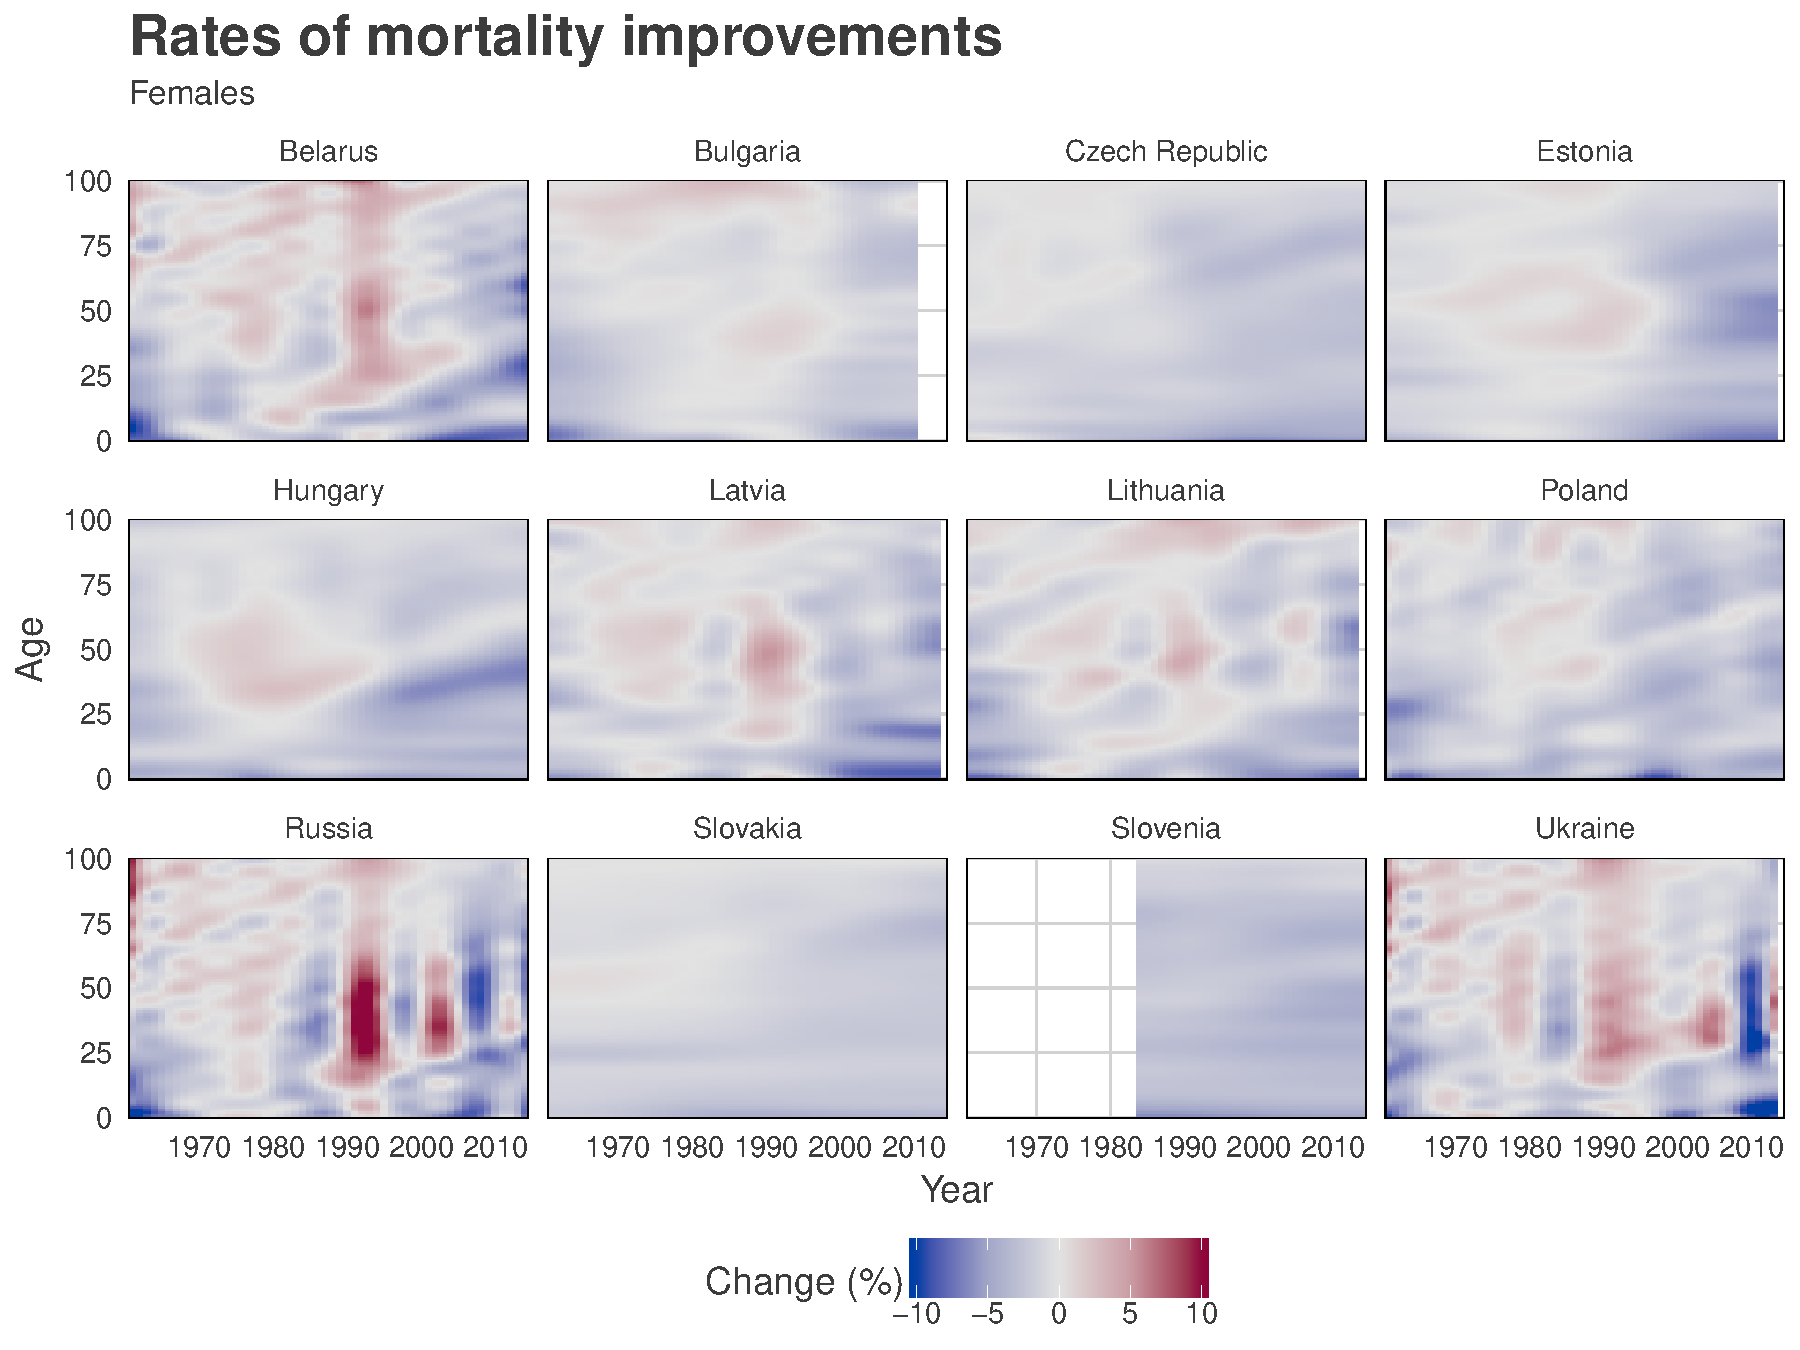
\includegraphics[scale=.55]{Figures/Romi_females.pdf}
\end{center}
Source: own calculations based on \citet{HMD} data. 
\begin{small}
Note: White areas indicate no data available
\end{small}
\end{figure}

\newpage

\begin{figure}[h!]
\centering
\caption{Trends in female life expectancy ($e_0$) and lifespan disparity  ($e^{\dagger}$) for 12 Eastern European countries, 1960-2014}
\begin{center}
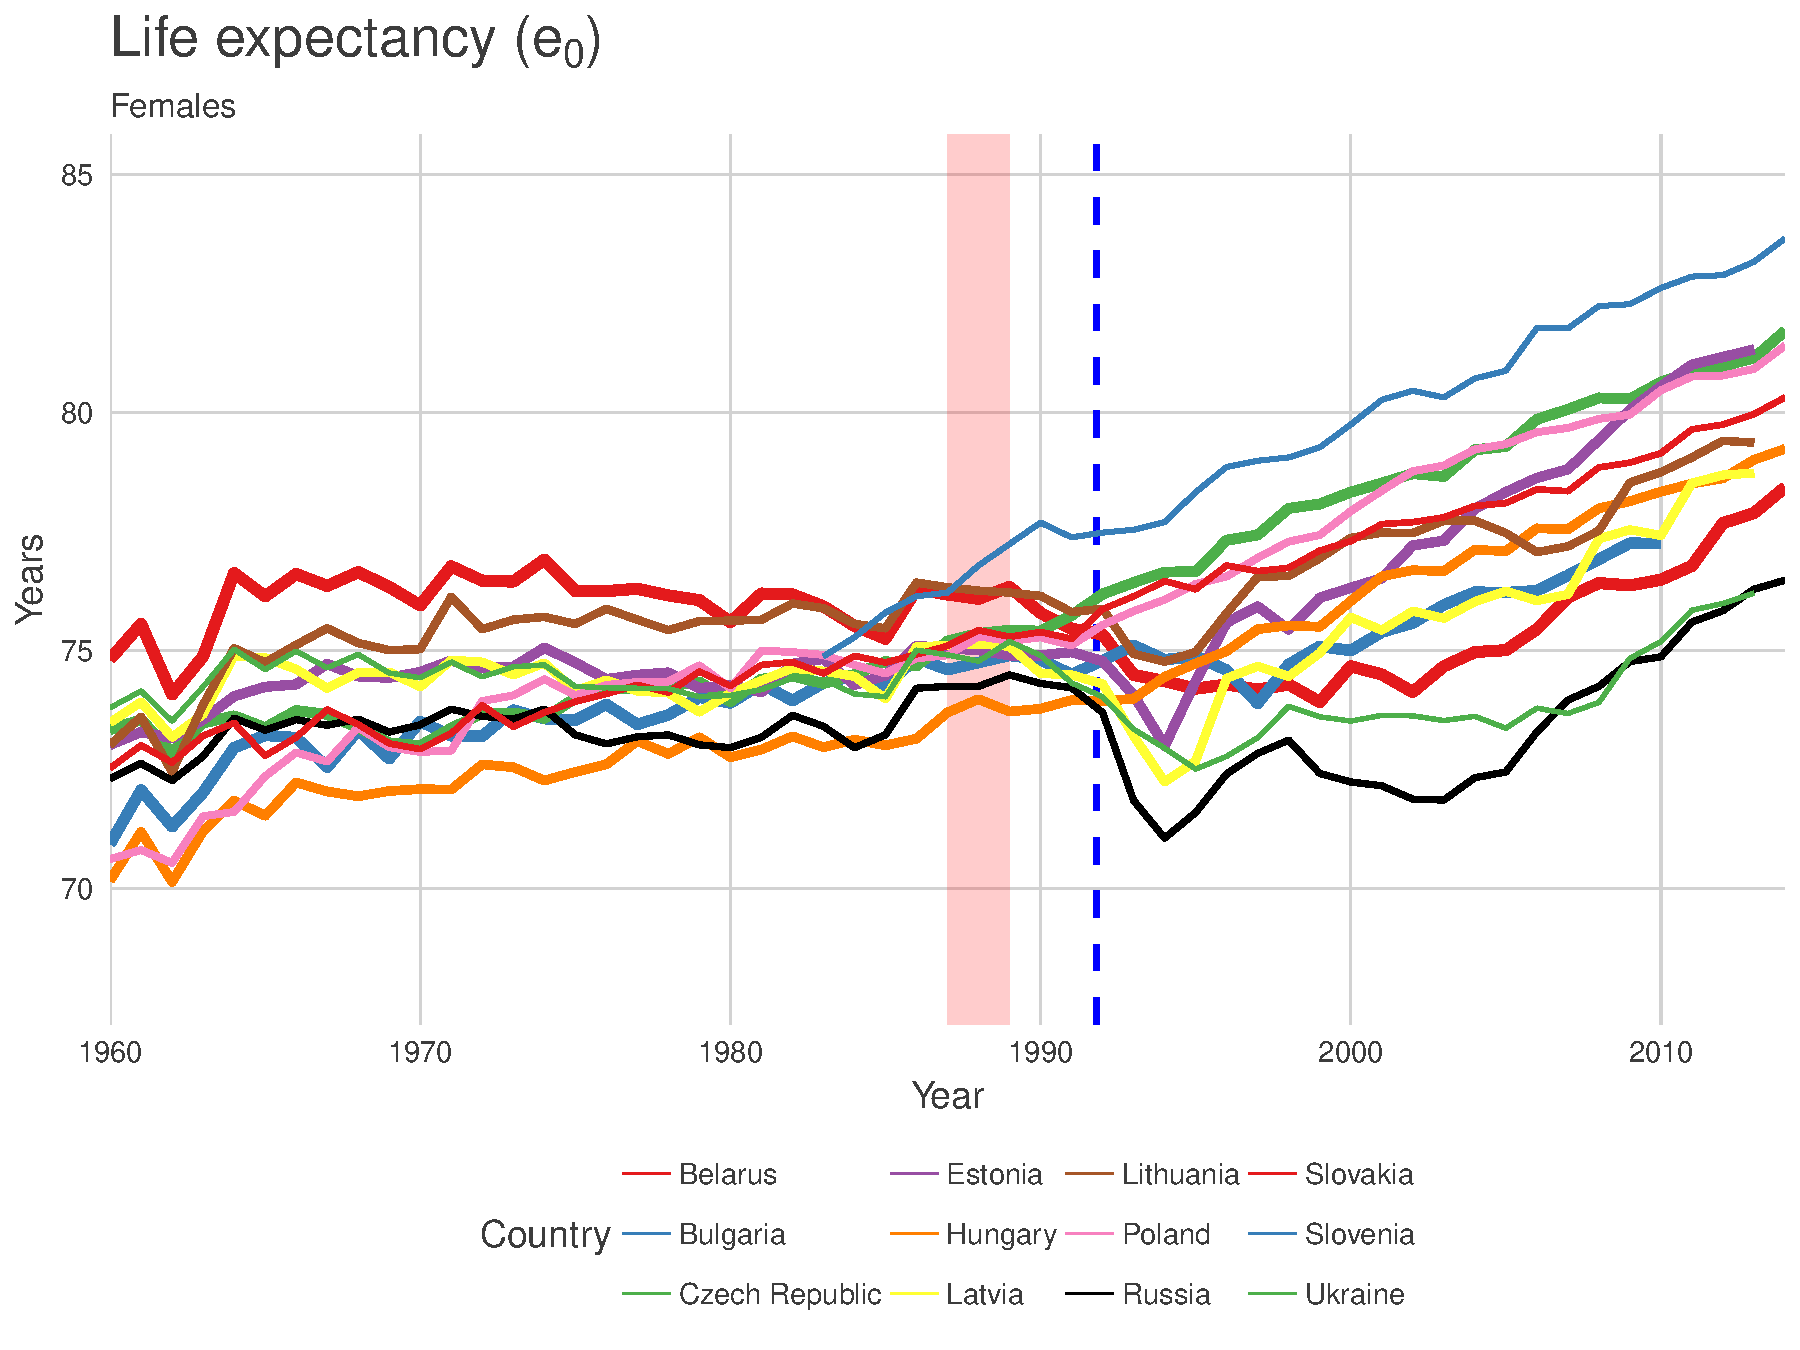
\includegraphics[scale=.40]{Figures/ex_females_labels.pdf}
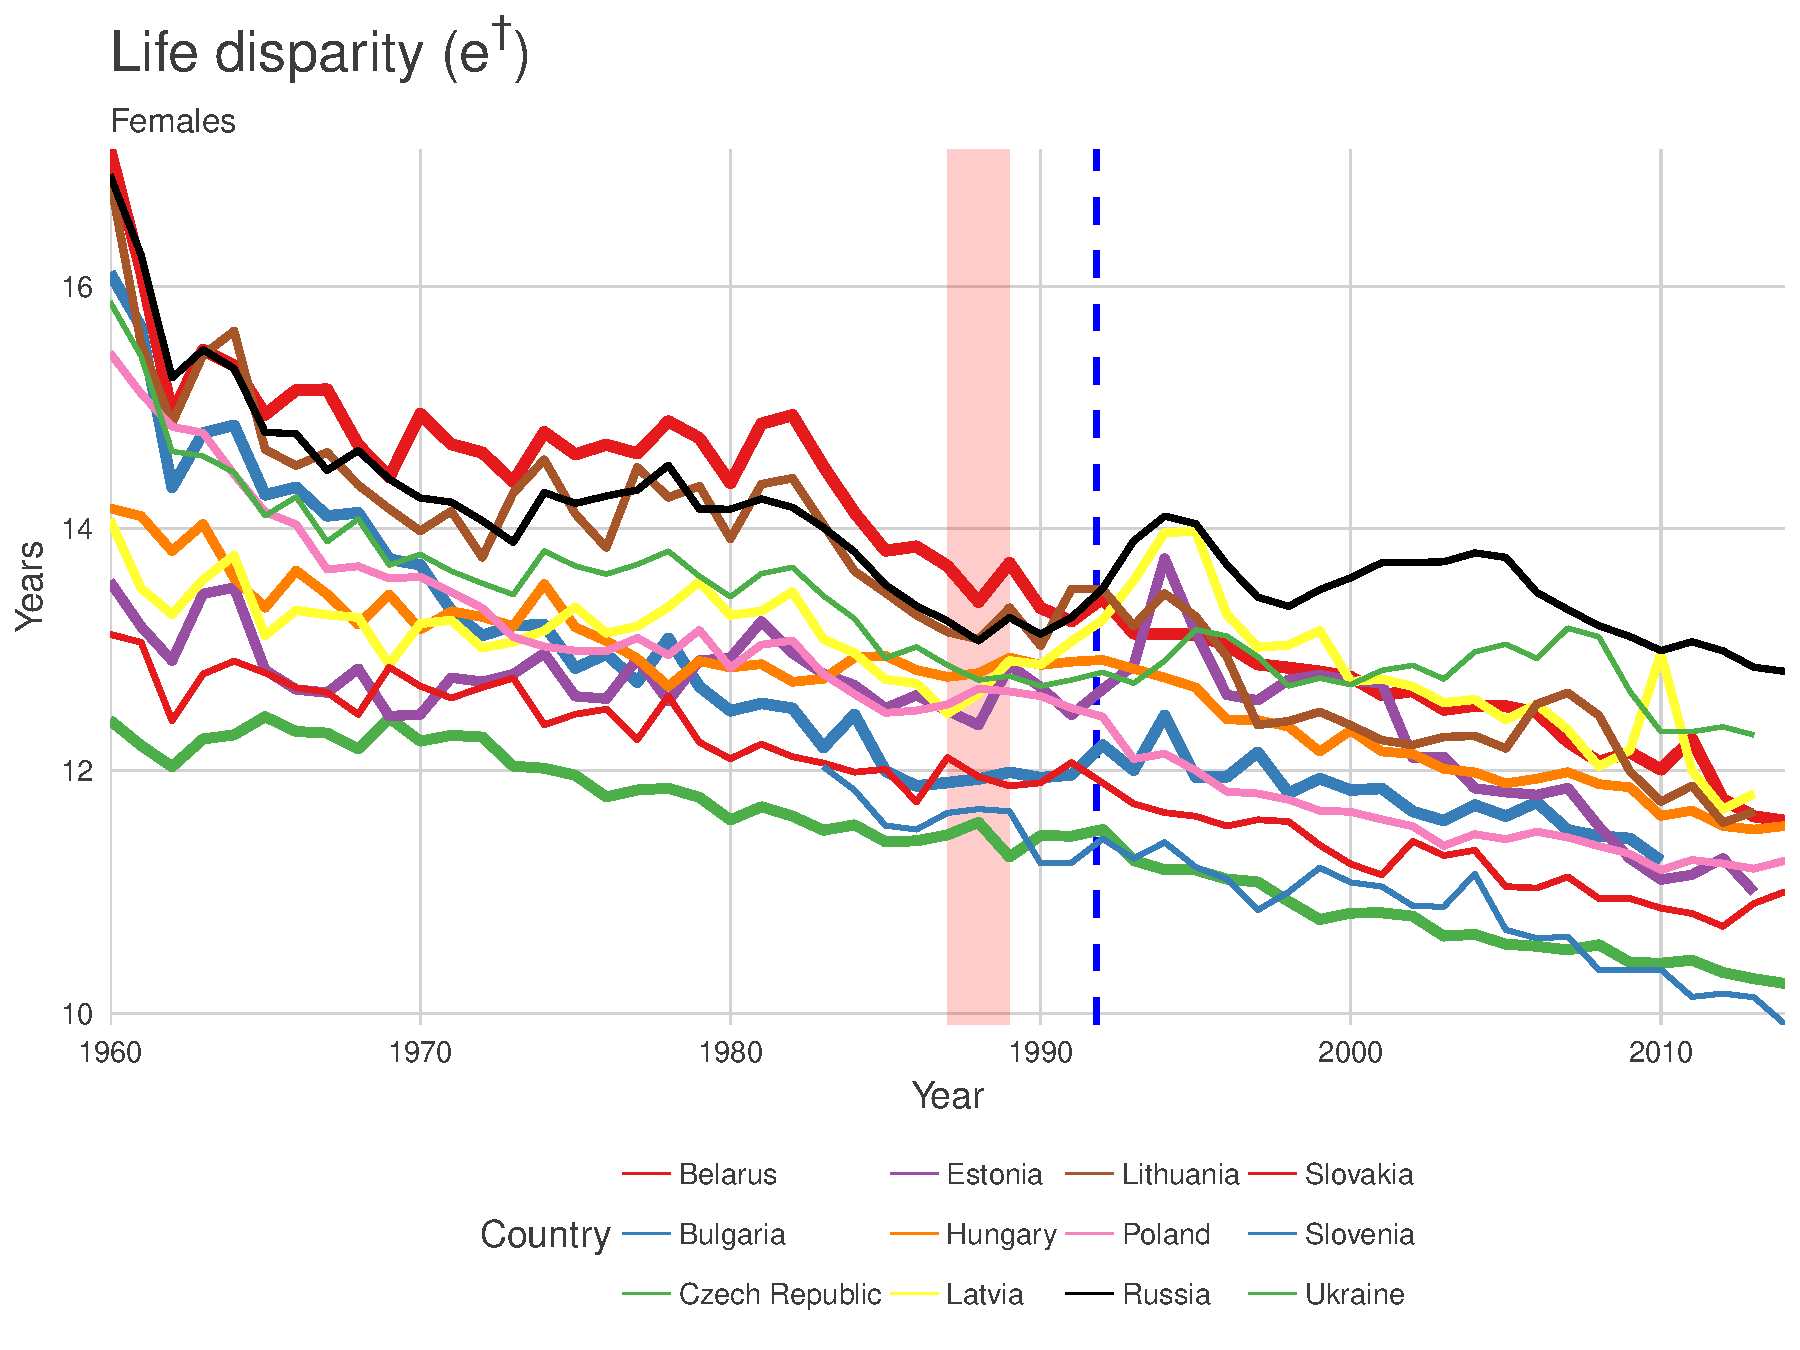
\includegraphics[scale=.40]{Figures/ed_females_labels.pdf}
\end{center}
Source: own calculations based on \citet{HMD} data. 
\end{figure}

\newpage

\begin{figure}[h!]
\centering
\caption{Absolute and relative yearly changes in life expectancy and lifespan disparity for females, 1960-2010}
\begin{center}
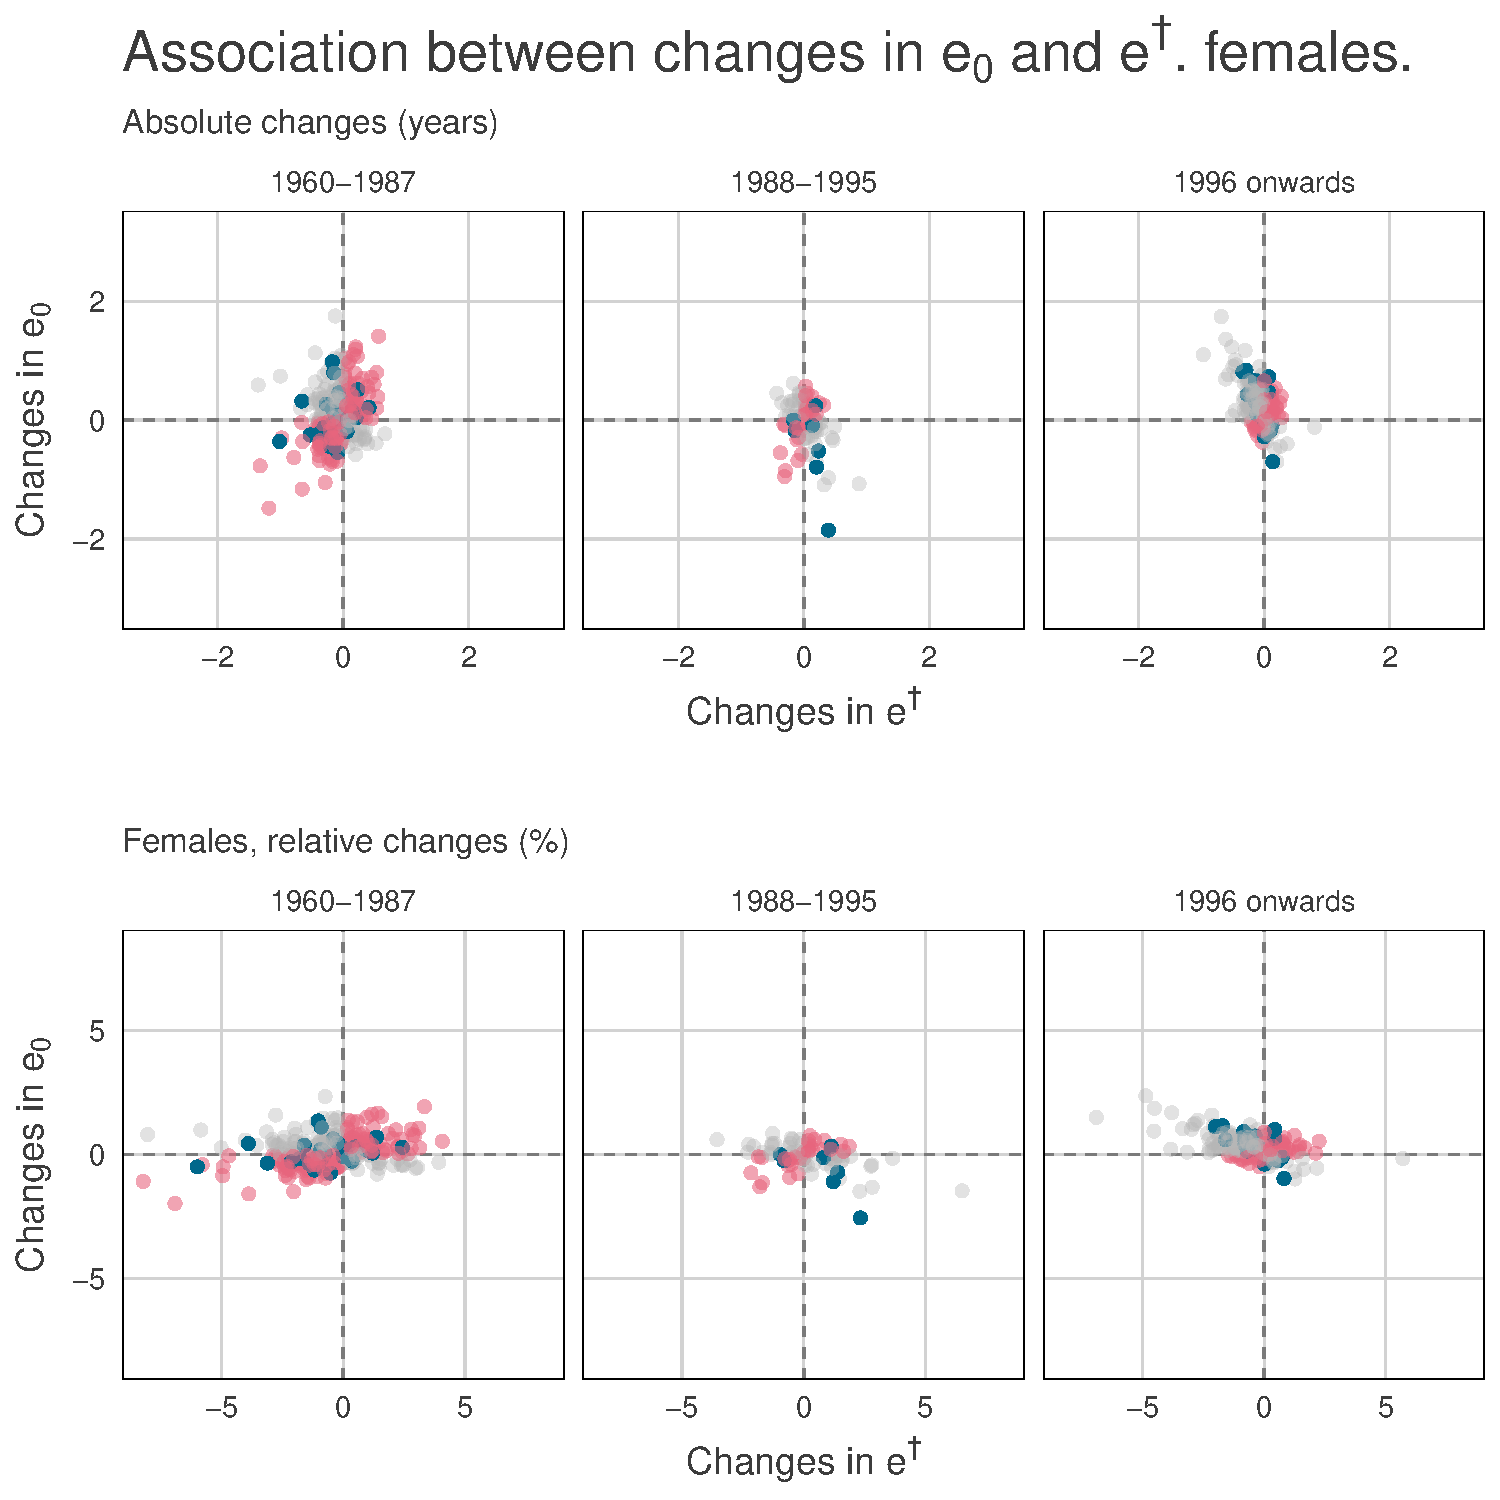
\includegraphics[scale=.65]{Figures/changes_females.pdf}
\end{center}
Source: own calculations based on \citet{HMD} data. Note: data for Slovenia begins in 1983. The dark dots are related to changes experienced in Russia.
\end{figure}

\newpage

\begin{figure}[h!]
\caption{Age-specific contributions to the change in lifespan disparity $e^\dagger$ by periods, females.}
\centering
\begin{center}
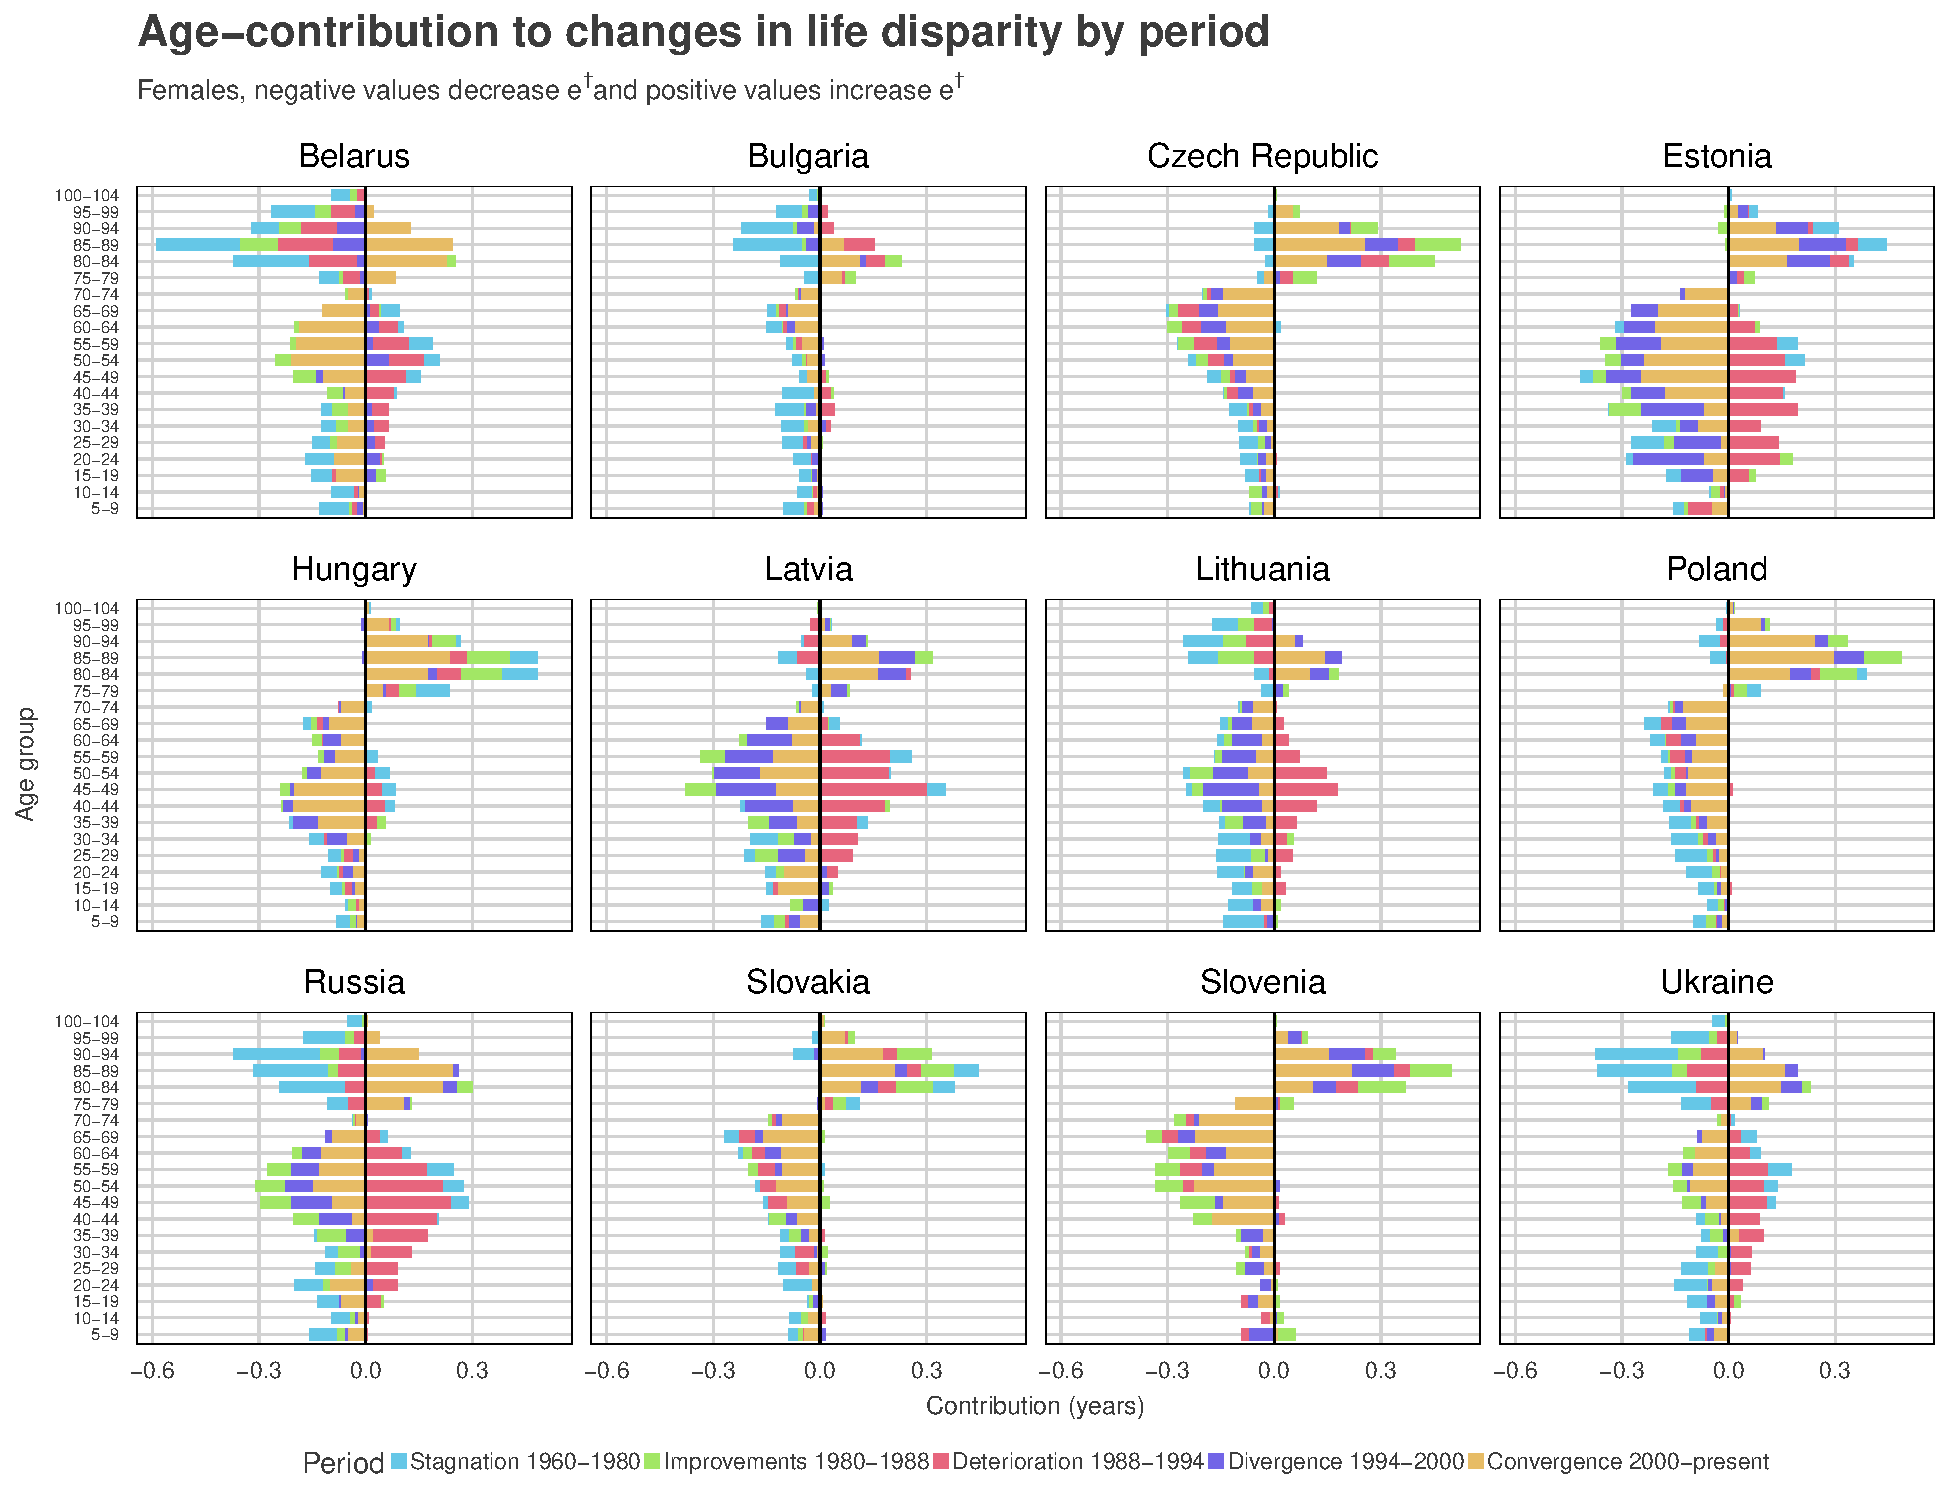
\includegraphics[scale=.46]{Figures/Age_ed_decomp_Females.pdf}
\end{center}
Source: own calculations based on \citet{HMD} data. Note: data for Slovenia begins in 1983.
\end{figure}

\newpage

\begin{figure}[h!]
\caption{Cause specific contributions to the change in  female lifespan disparity  $e^\dagger$, 1994-2000}
\centering
\begin{center}
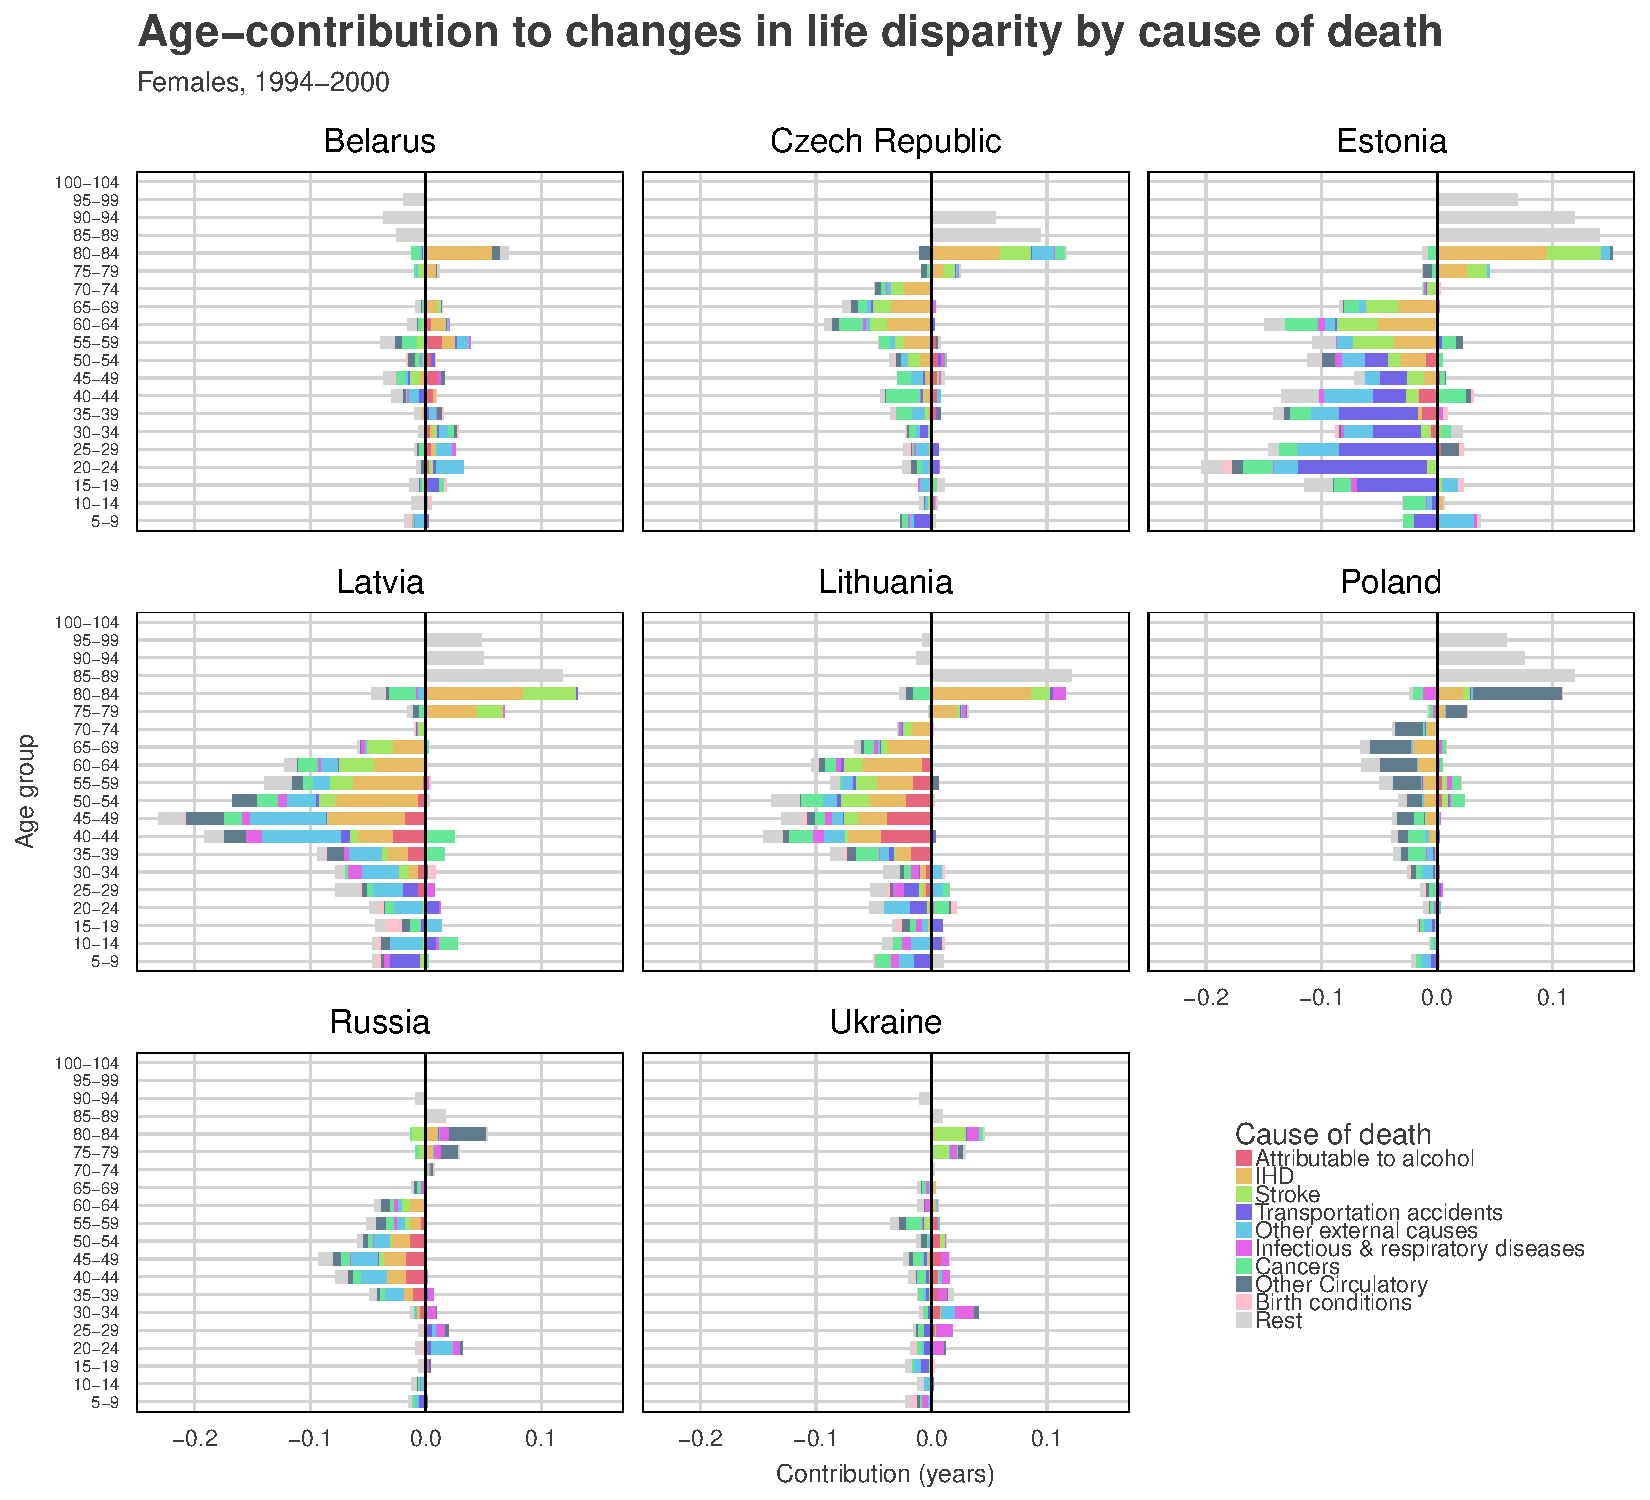
\includegraphics[scale=.5]{Figures/Cause_ed_decomp_Females_1.pdf}
\end{center}
Source: own calculations based on \citet{HMD} data. 
\end{figure}

\newpage

\begin{figure}[h!]
\caption{Cause specific contributions to the change in  female lifespan disparity  $e^\dagger$, 2000-2010}
\centering
\begin{center}
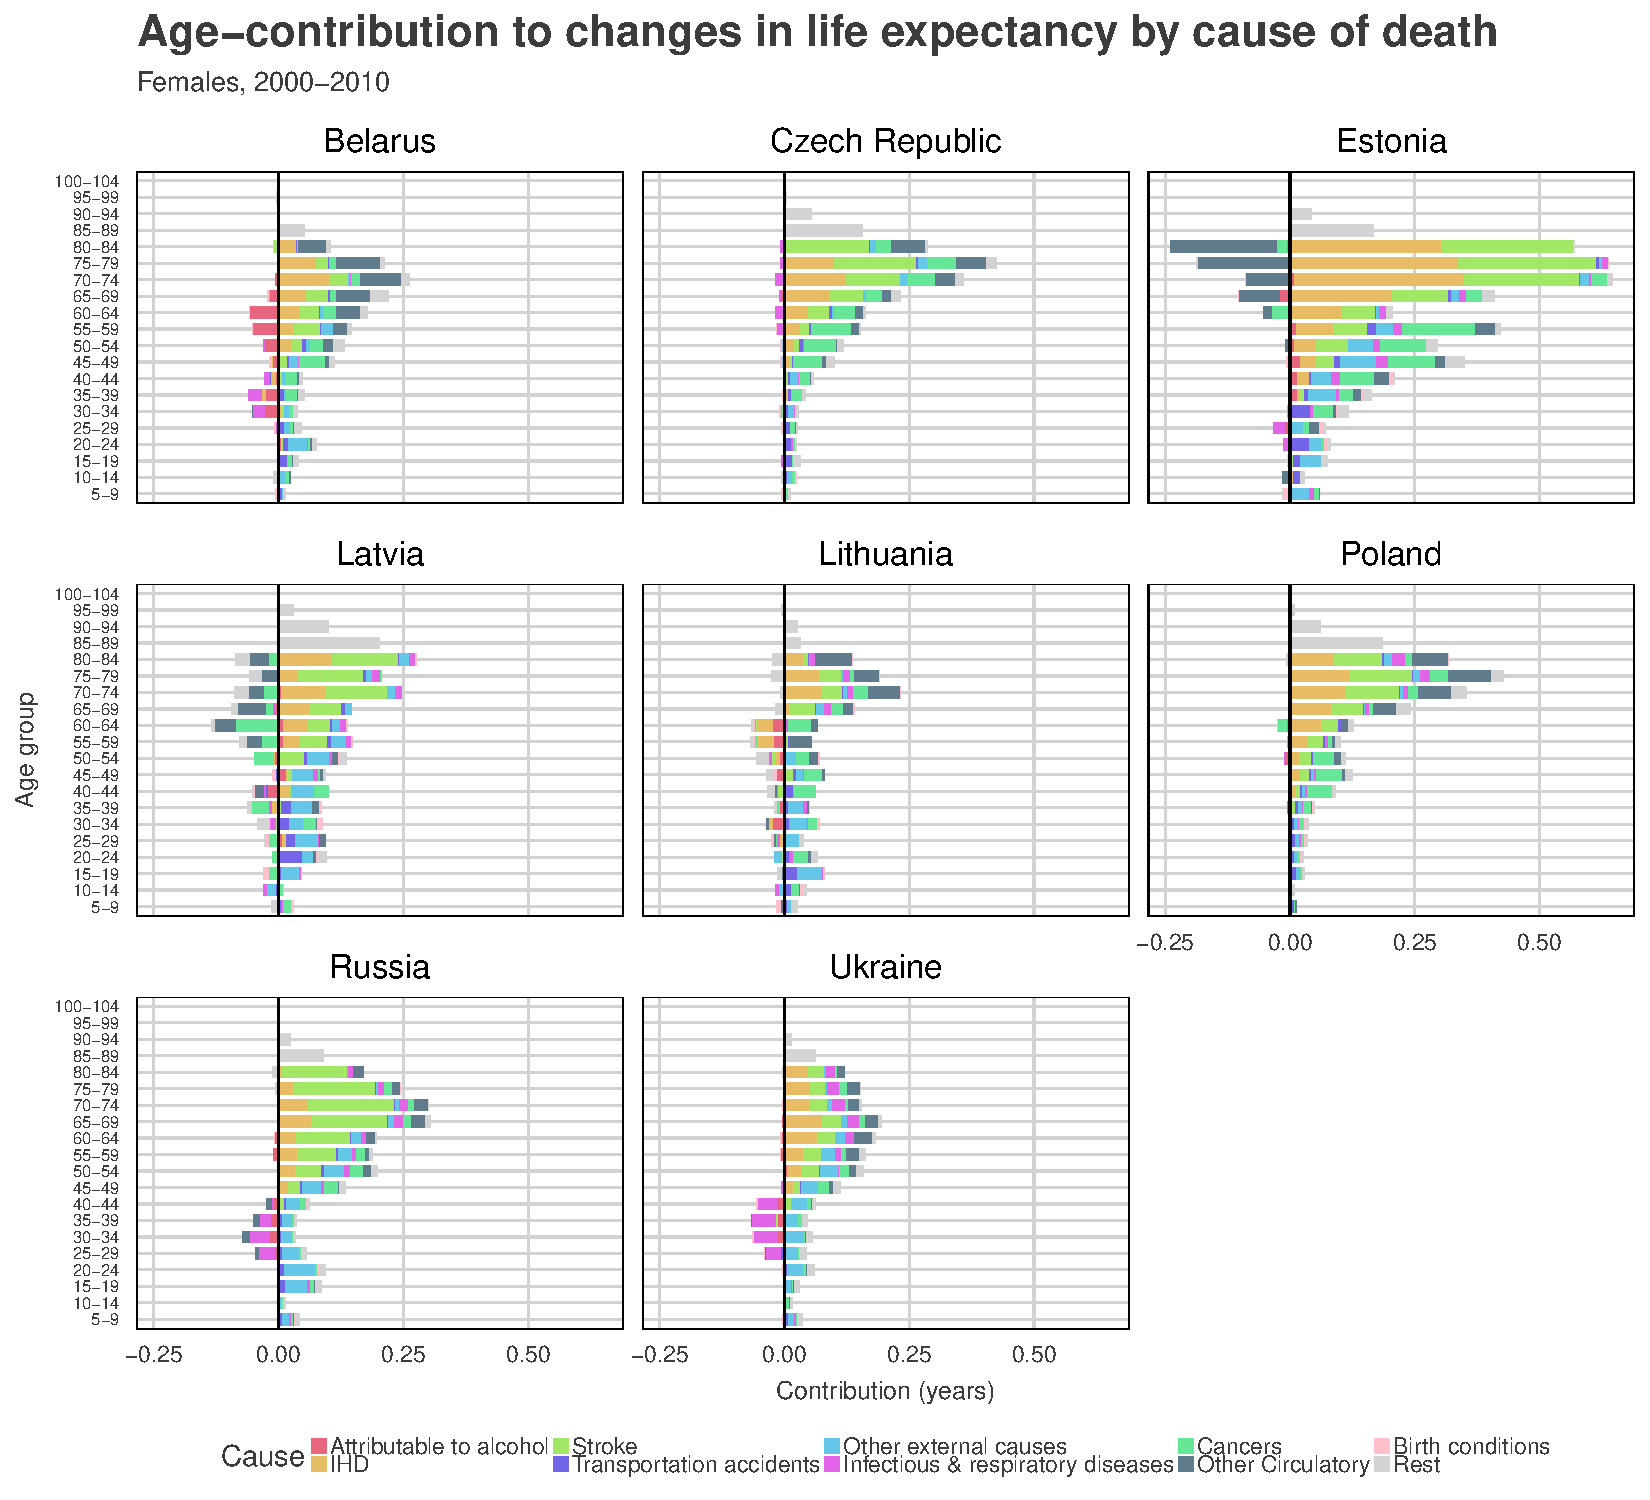
\includegraphics[scale=.5]{Figures/Cause_ed_decomp_Females_2.pdf}
\end{center}
Source: own calculations based on \citet{HMD} data. Note: data for Poland ends in 2009.
\end{figure}

\newpage



\section*{Infant contributions to changes in $e^\dagger$ and $e_0$}

\begin{figure}[h!]
\centering
\caption{Infant contributions, below age 5, to changes in $e^\dagger$ and $e_0$ by period and sex}
\label{Fig_LE&LD}
\begin{center}
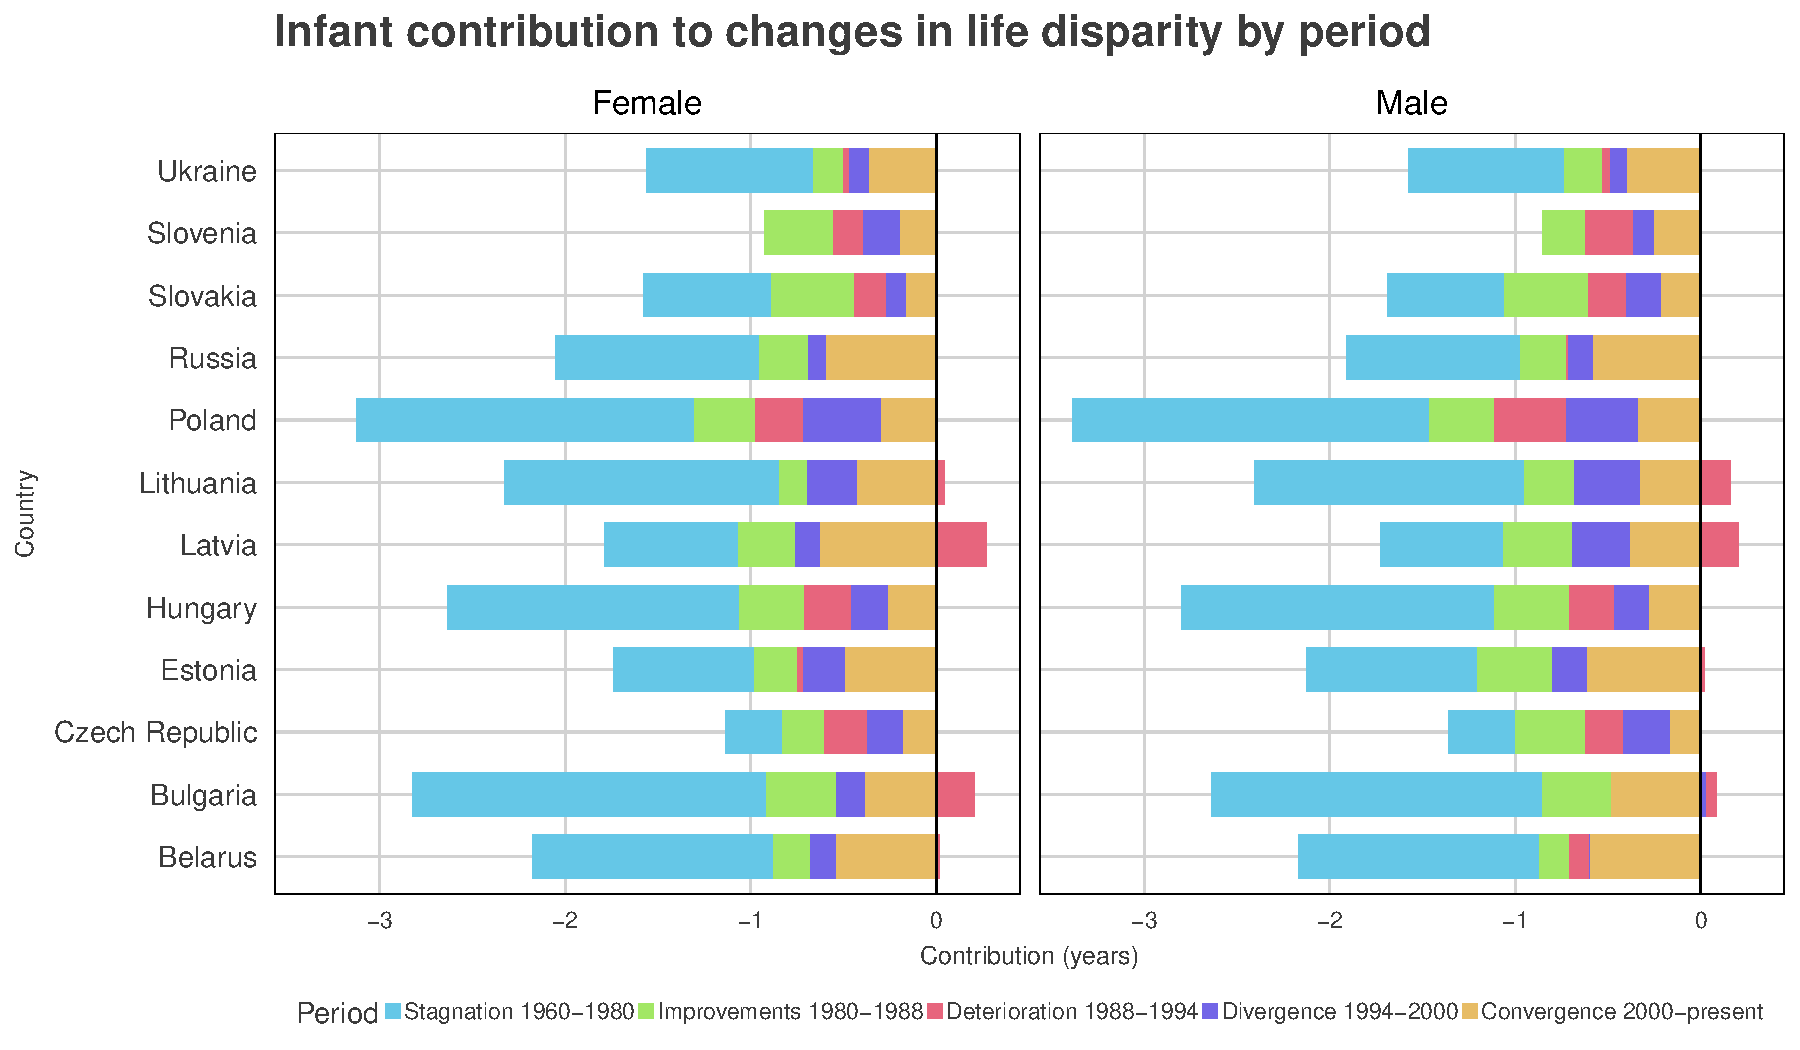
\includegraphics[scale=.5]{Figures/Infant_ed_decomp.pdf}
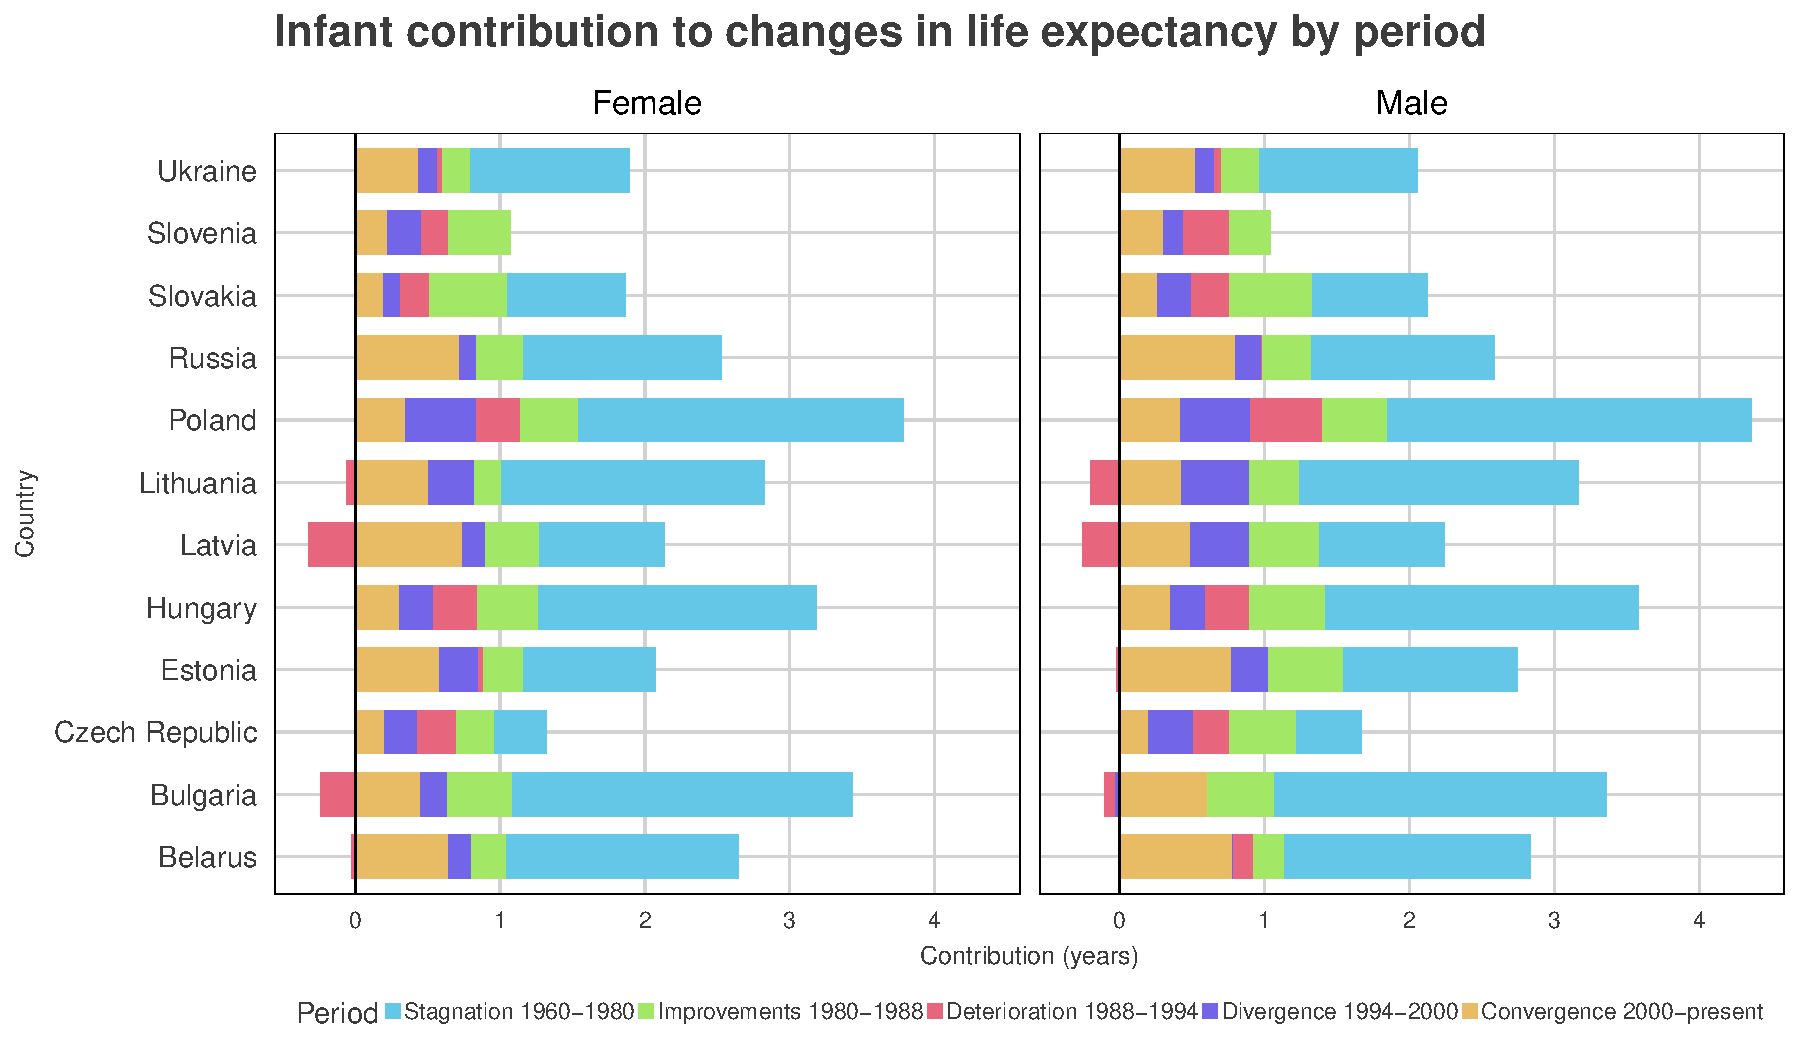
\includegraphics[scale=.5]{Figures/Infant_ex_decomp.pdf}
\end{center}
Source: own calculations based on \citet{HMD} data. 
\end{figure}

\newpage

\section*{Age and age-cause specific decomposition results for life expectancy}


\begin{figure}[h!]
\caption{Age-specific contributions to the change in $e_0$ by periods for males.}
\centering
\begin{center}
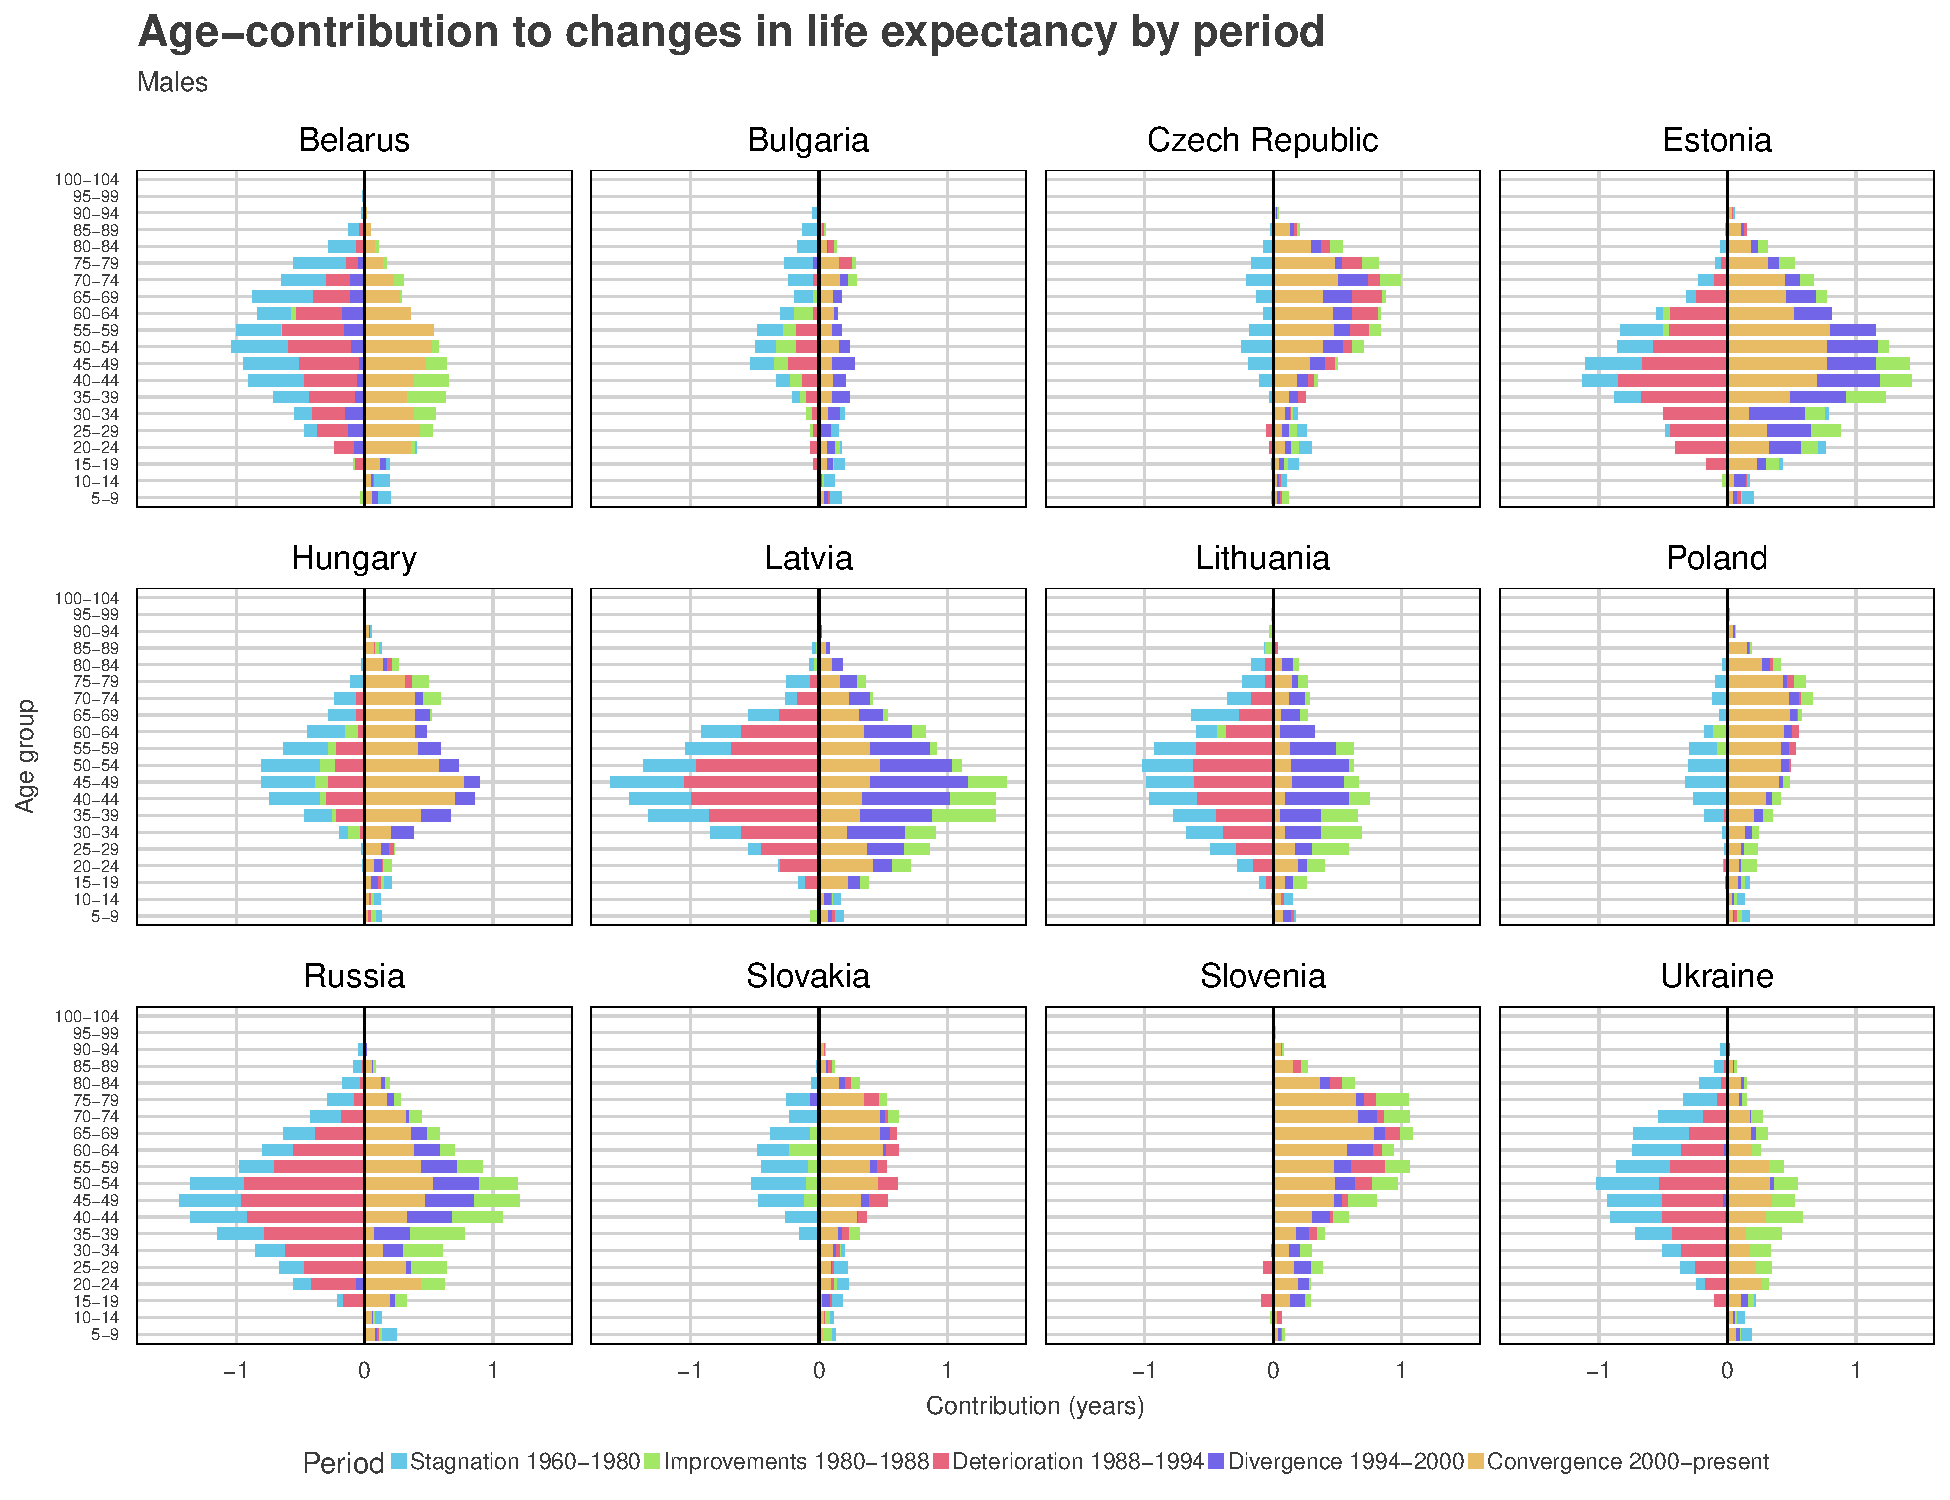
\includegraphics[scale=.46]{Figures/Age_e0_decomp_Males.pdf}
\end{center}
Source: own calculations based on \citet{HMD} data. Note: data for Slovenia begins in 1983.
\end{figure}

\newpage

\begin{figure}[h!]
\caption{Age-specific contributions to the change in $e_0$ by periods for females.}
\centering
\begin{center}
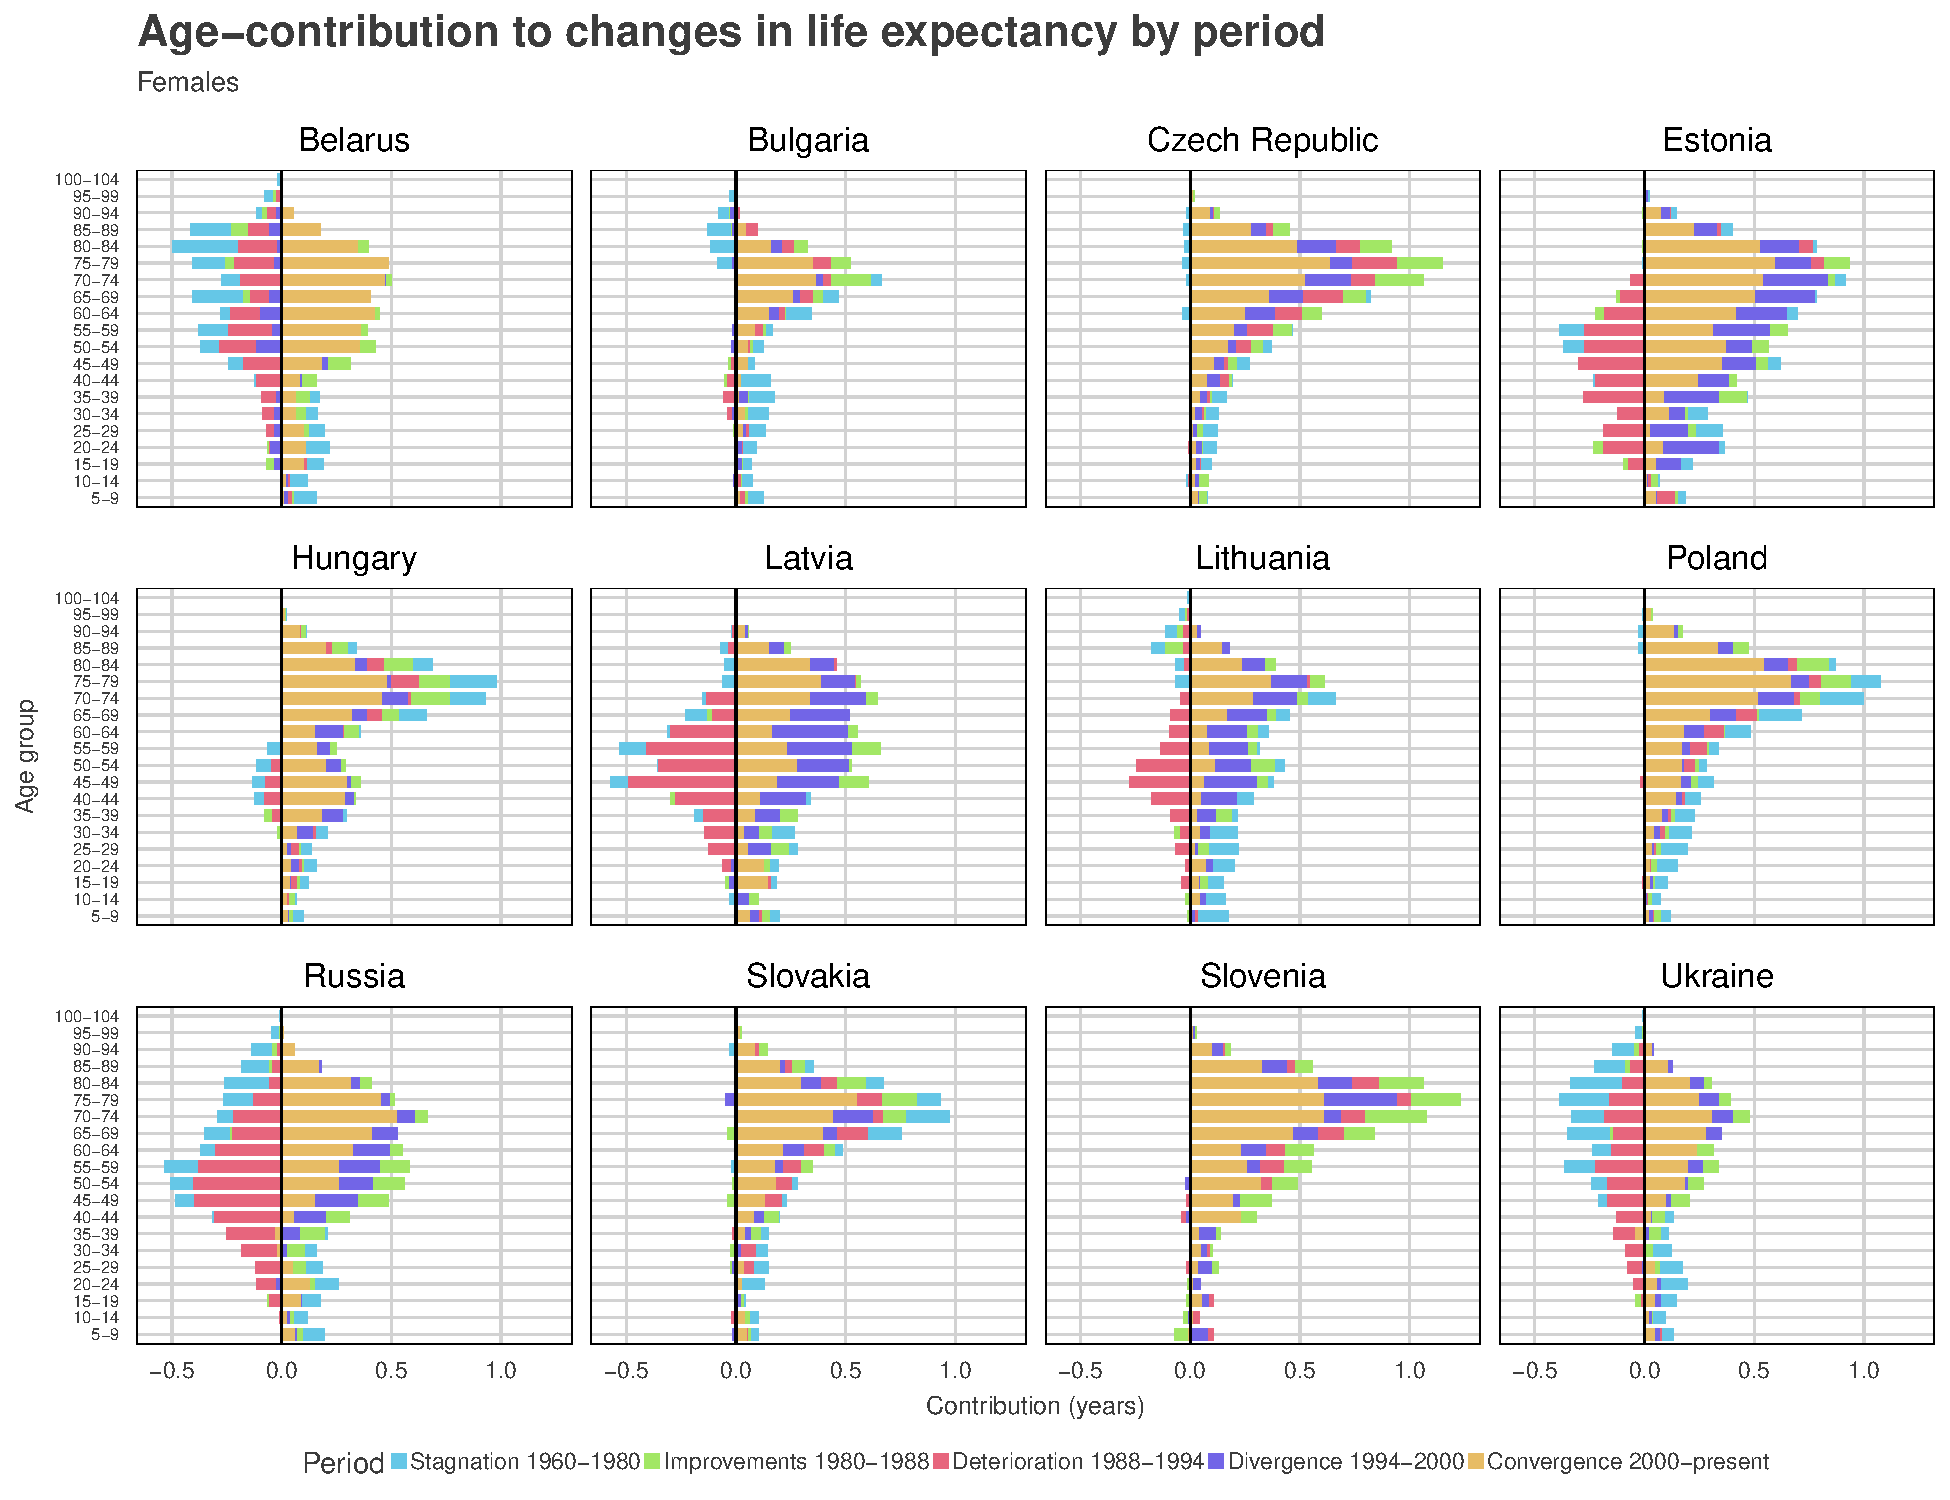
\includegraphics[scale=.46]{Figures/Age_e0_decomp_Females.pdf}
\end{center}
Source: own calculations based on \citet{HMD} data. Note: data for Slovenia begins in 1983.
\end{figure}

\newpage

\begin{figure}[h!]
\caption{Age-cause-specific contributions to the change in $e_0$ by periods for males 1994-2000.}
\centering
\begin{center}
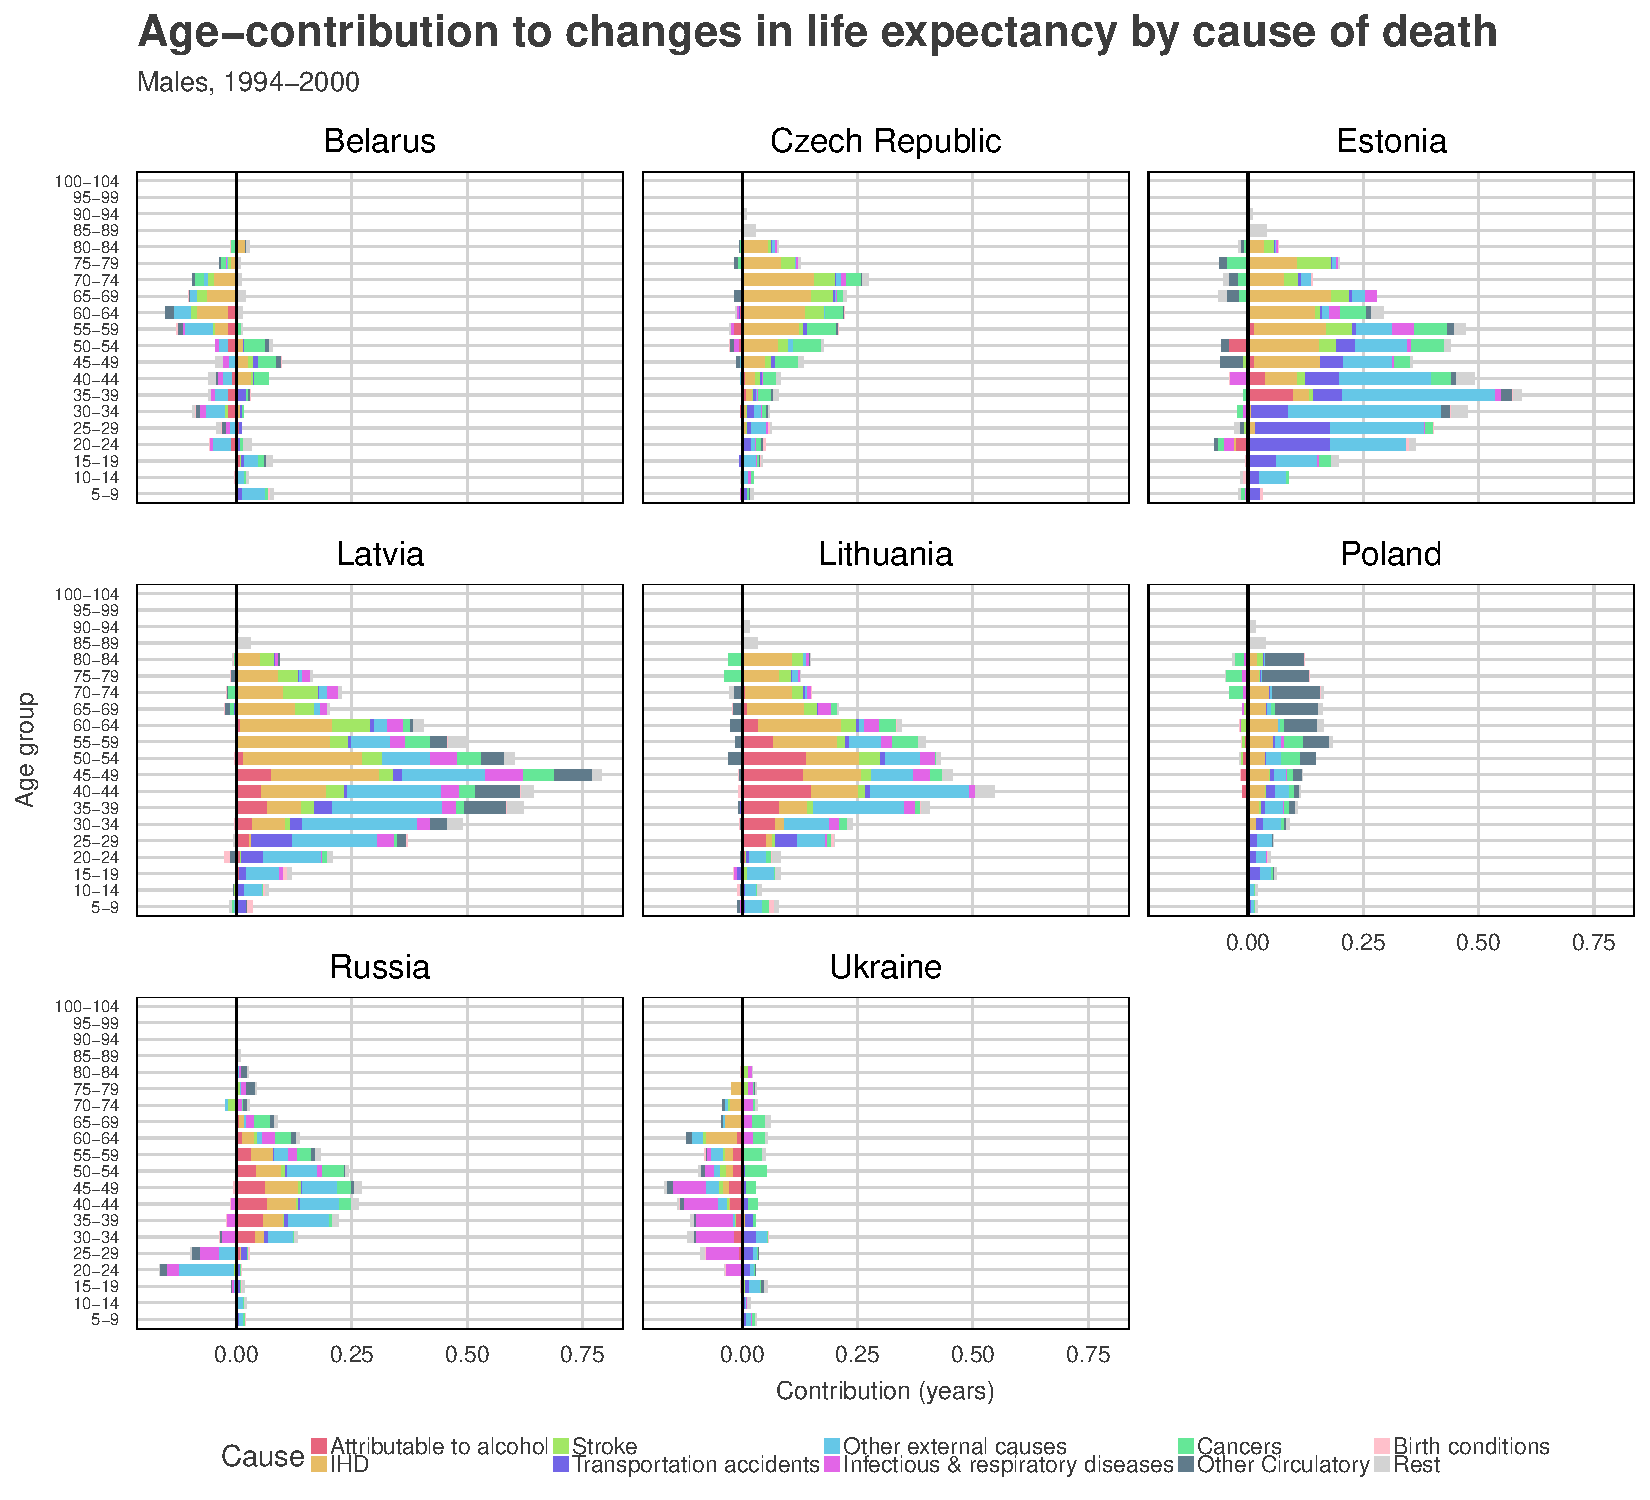
\includegraphics[scale=.5]{Figures/Cause_e0_decomp_Males_1.pdf}
\end{center}
Source: own calculations based on \citet{HMD} data. Note: data for Slovenia begins in 1983.
\end{figure}

\newpage
\begin{figure}[h!]
\caption{Age-cause-specific contributions to the change in $e_0$ by periods for males 2000-2010.}
\centering
\begin{center}
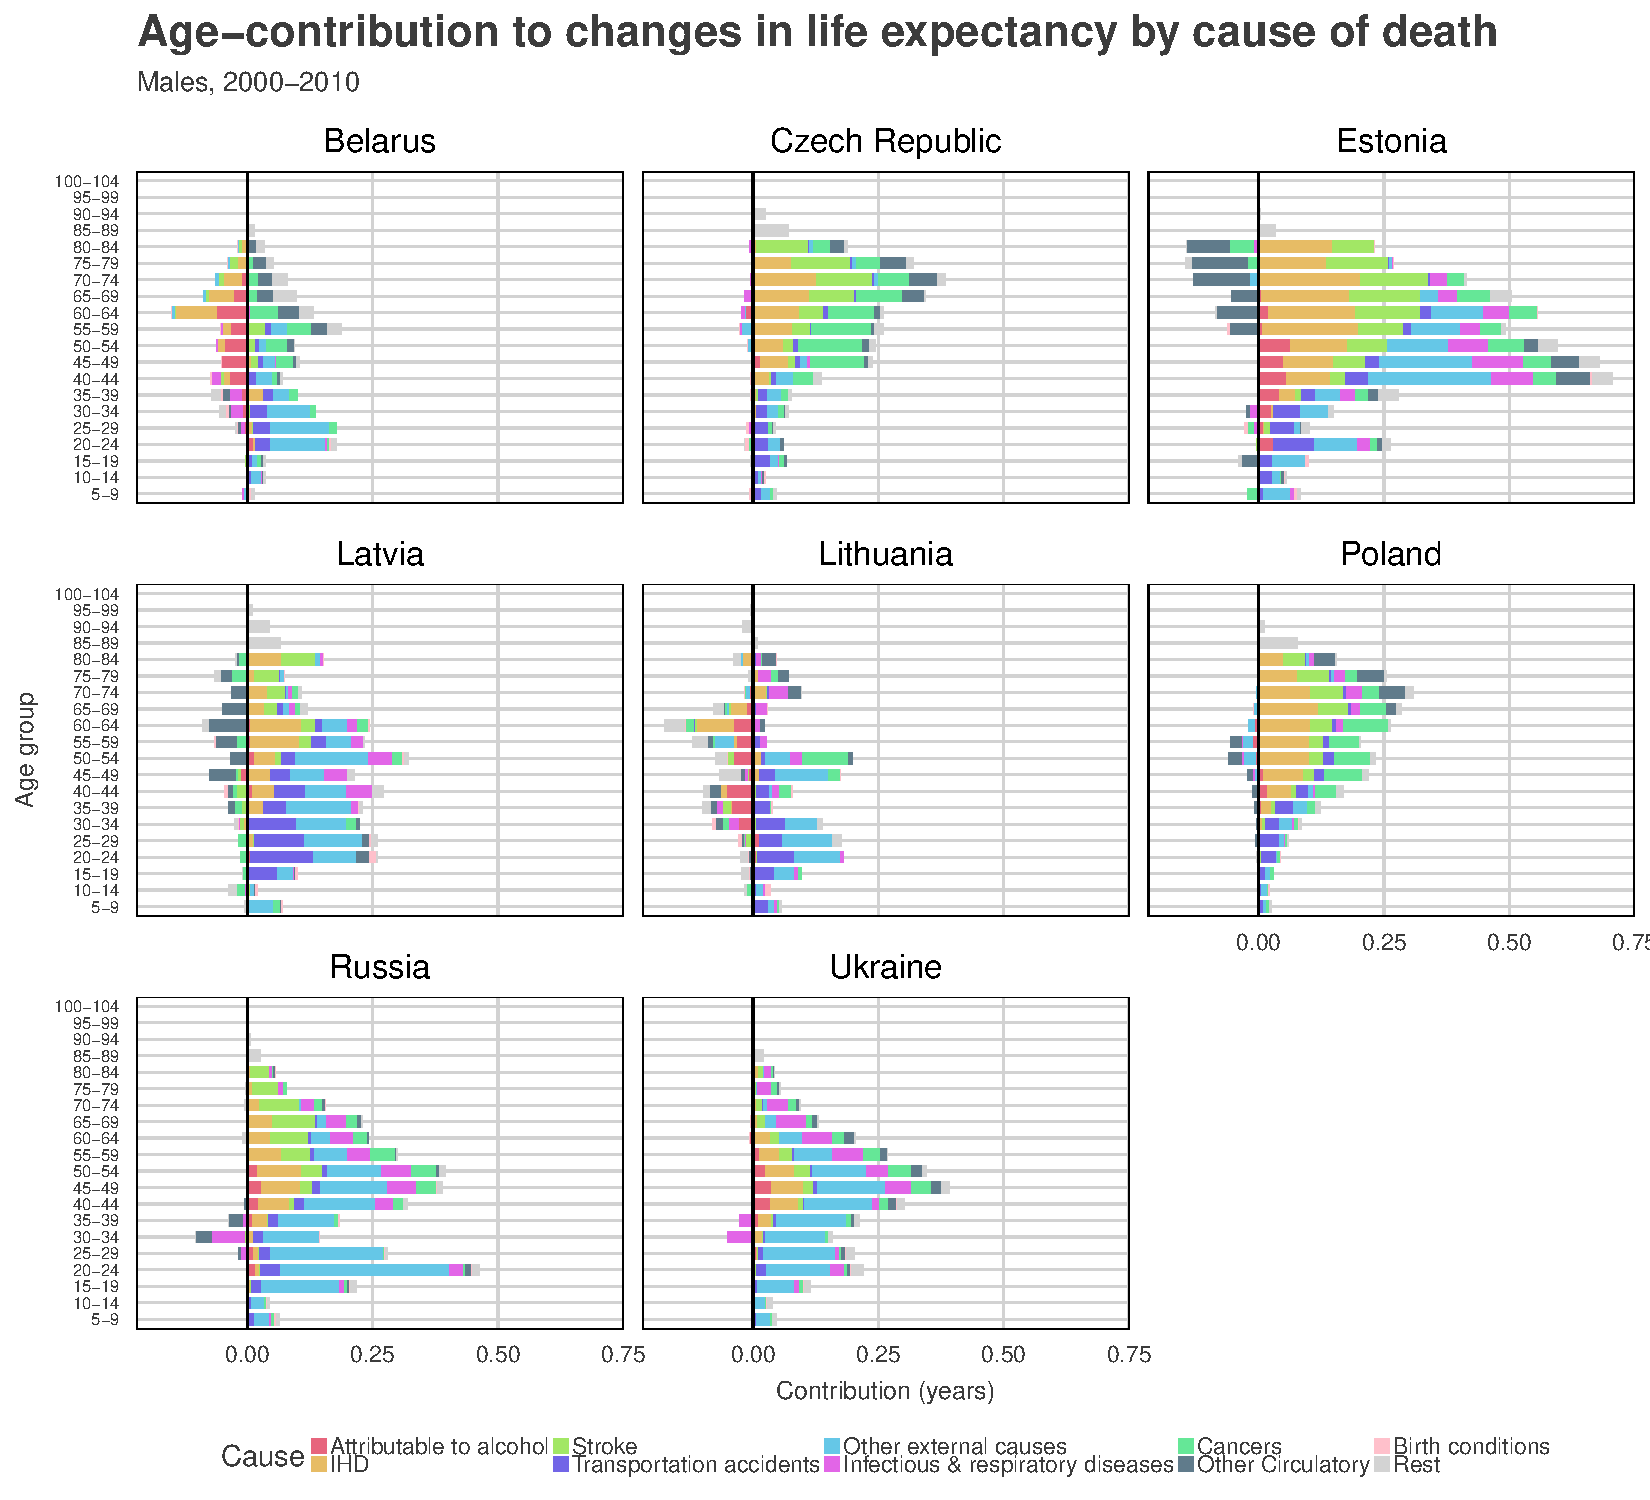
\includegraphics[scale=.5]{Figures/Cause_e0_decomp_Males_2.pdf}
\end{center}
Source: own calculations based on \citet{HMD} data. Note: data for Slovenia begins in 1983.
\end{figure}

\newpage

\begin{figure}[h!]
\caption{Age-cause-specific contributions to the change in $e_0$ by periods for females 1994-2000.}
\centering
\begin{center}
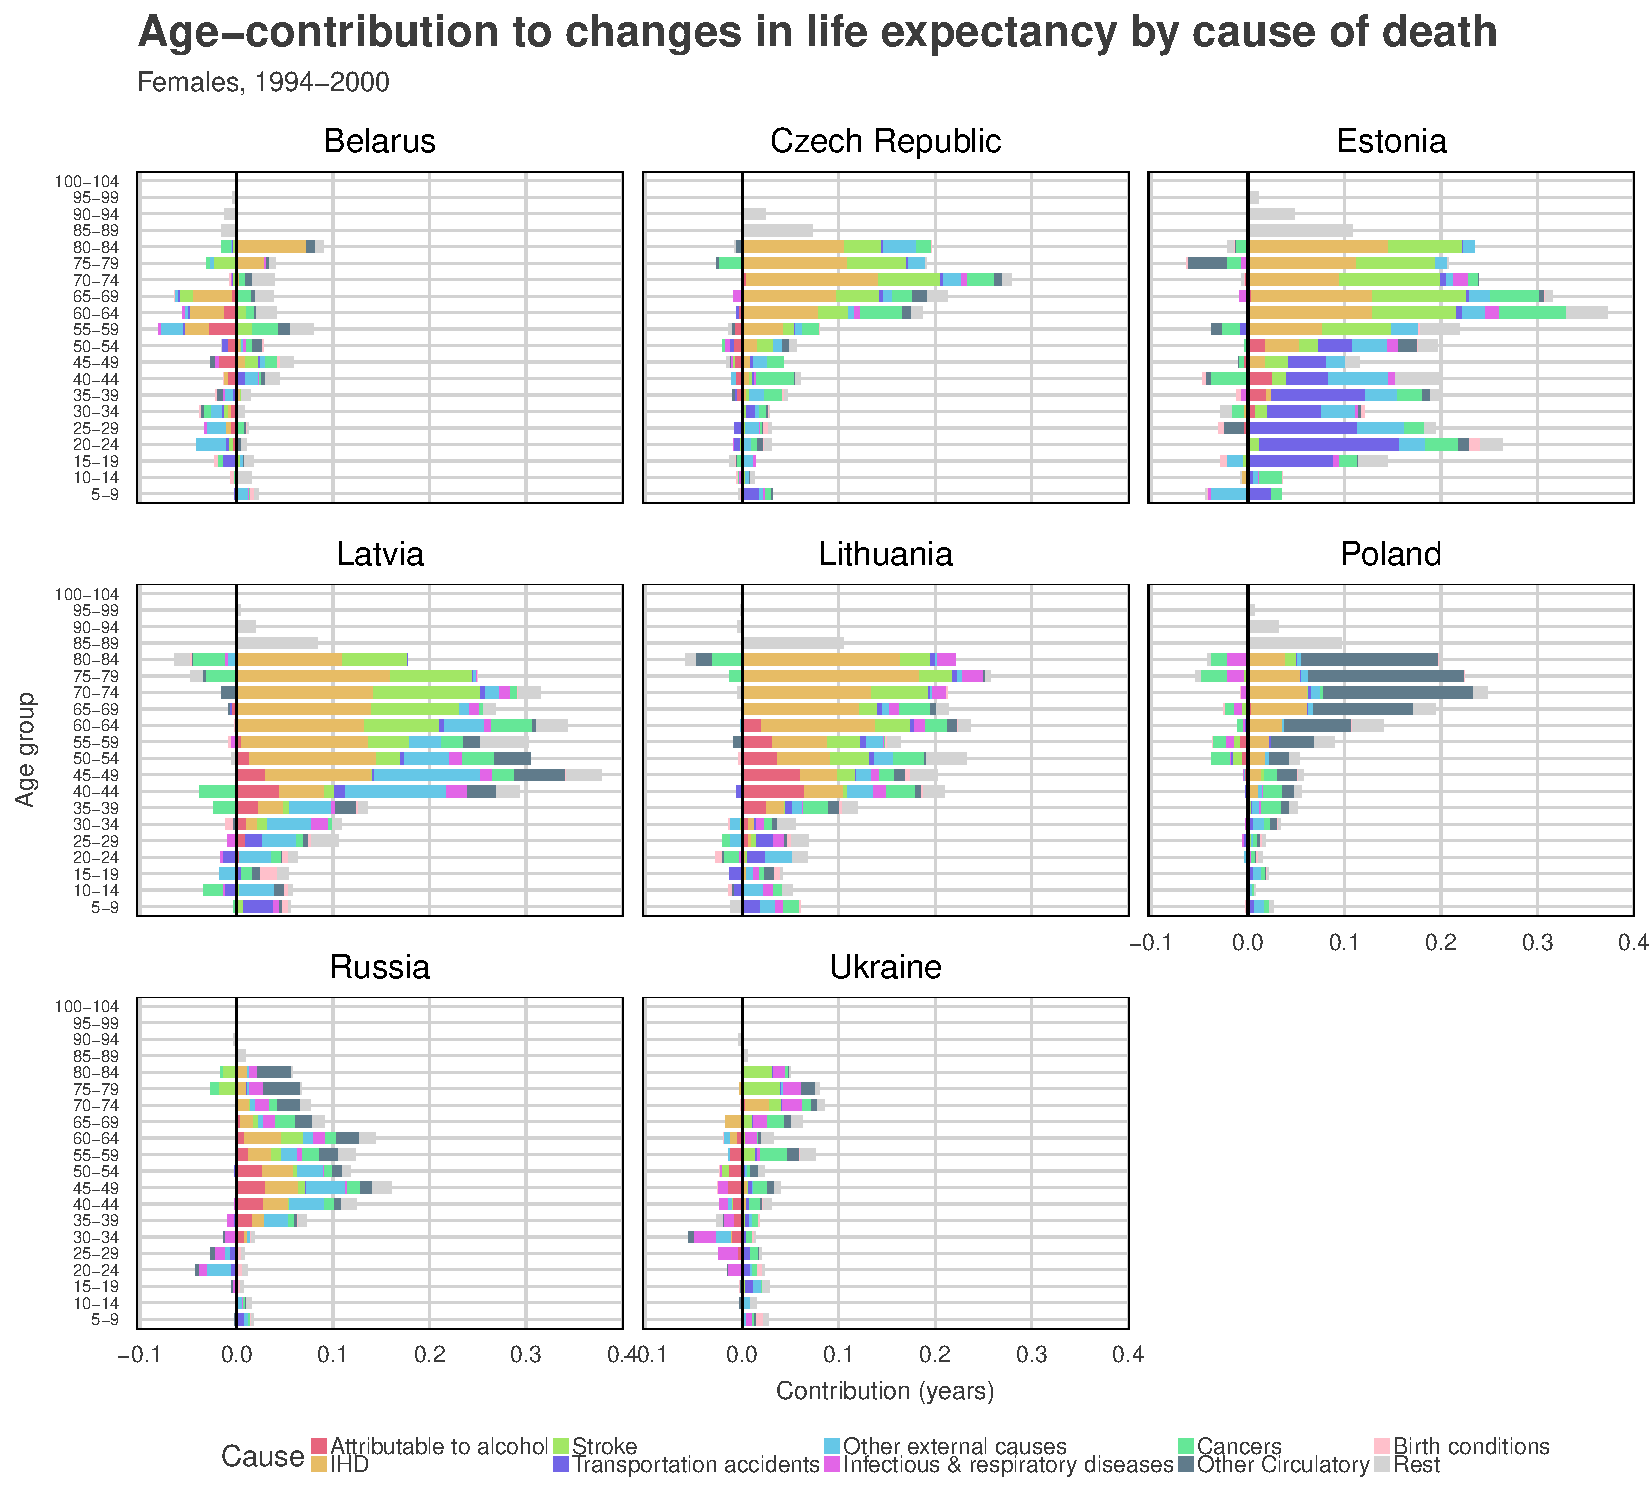
\includegraphics[scale=.5]{Figures/Cause_e0_decomp_Females_1.pdf}
\end{center}
Source: own calculations based on \citet{HMD} data. Note: data for Slovenia begins in 1983.
\end{figure}

\newpage

\begin{figure}[h!]
\caption{Age-cause-specific contributions to the change in $e_0$ by periods for females 2000-2010.}
\centering
\begin{center}
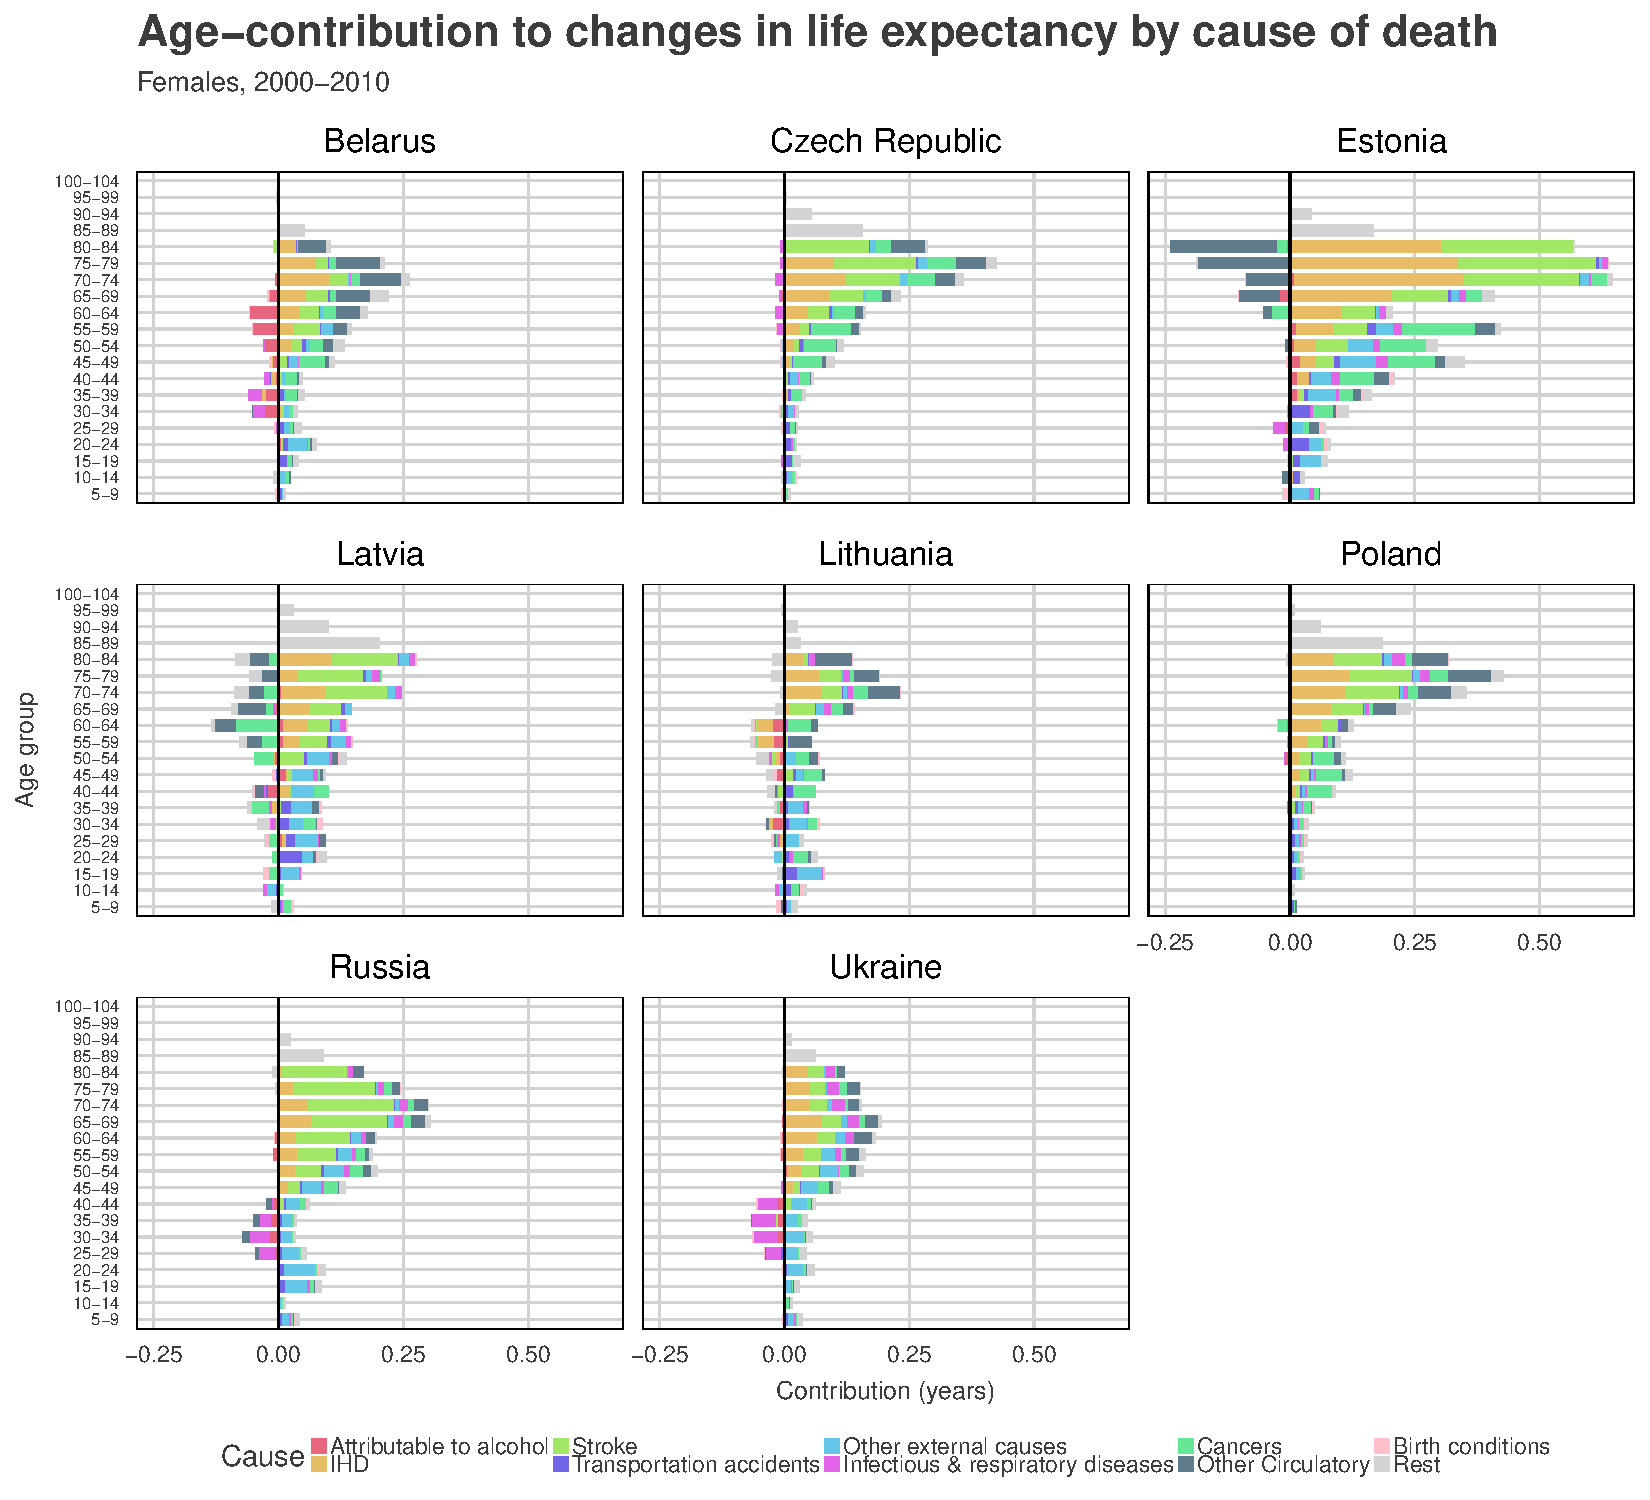
\includegraphics[scale=.5]{Figures/Cause_e0_decomp_Females_2.pdf}
\end{center}
Source: own calculations based on \citet{HMD} data. Note: data for Slovenia begins in 1983.
\end{figure}

\newpage
\section*{Sensitivity analysis with the Gini coefficient}

\begin{figure}[h!]
\caption{Trends in life expectancy and Gini coefficient by sex for Eastern European countries}
\centering
\begin{center}
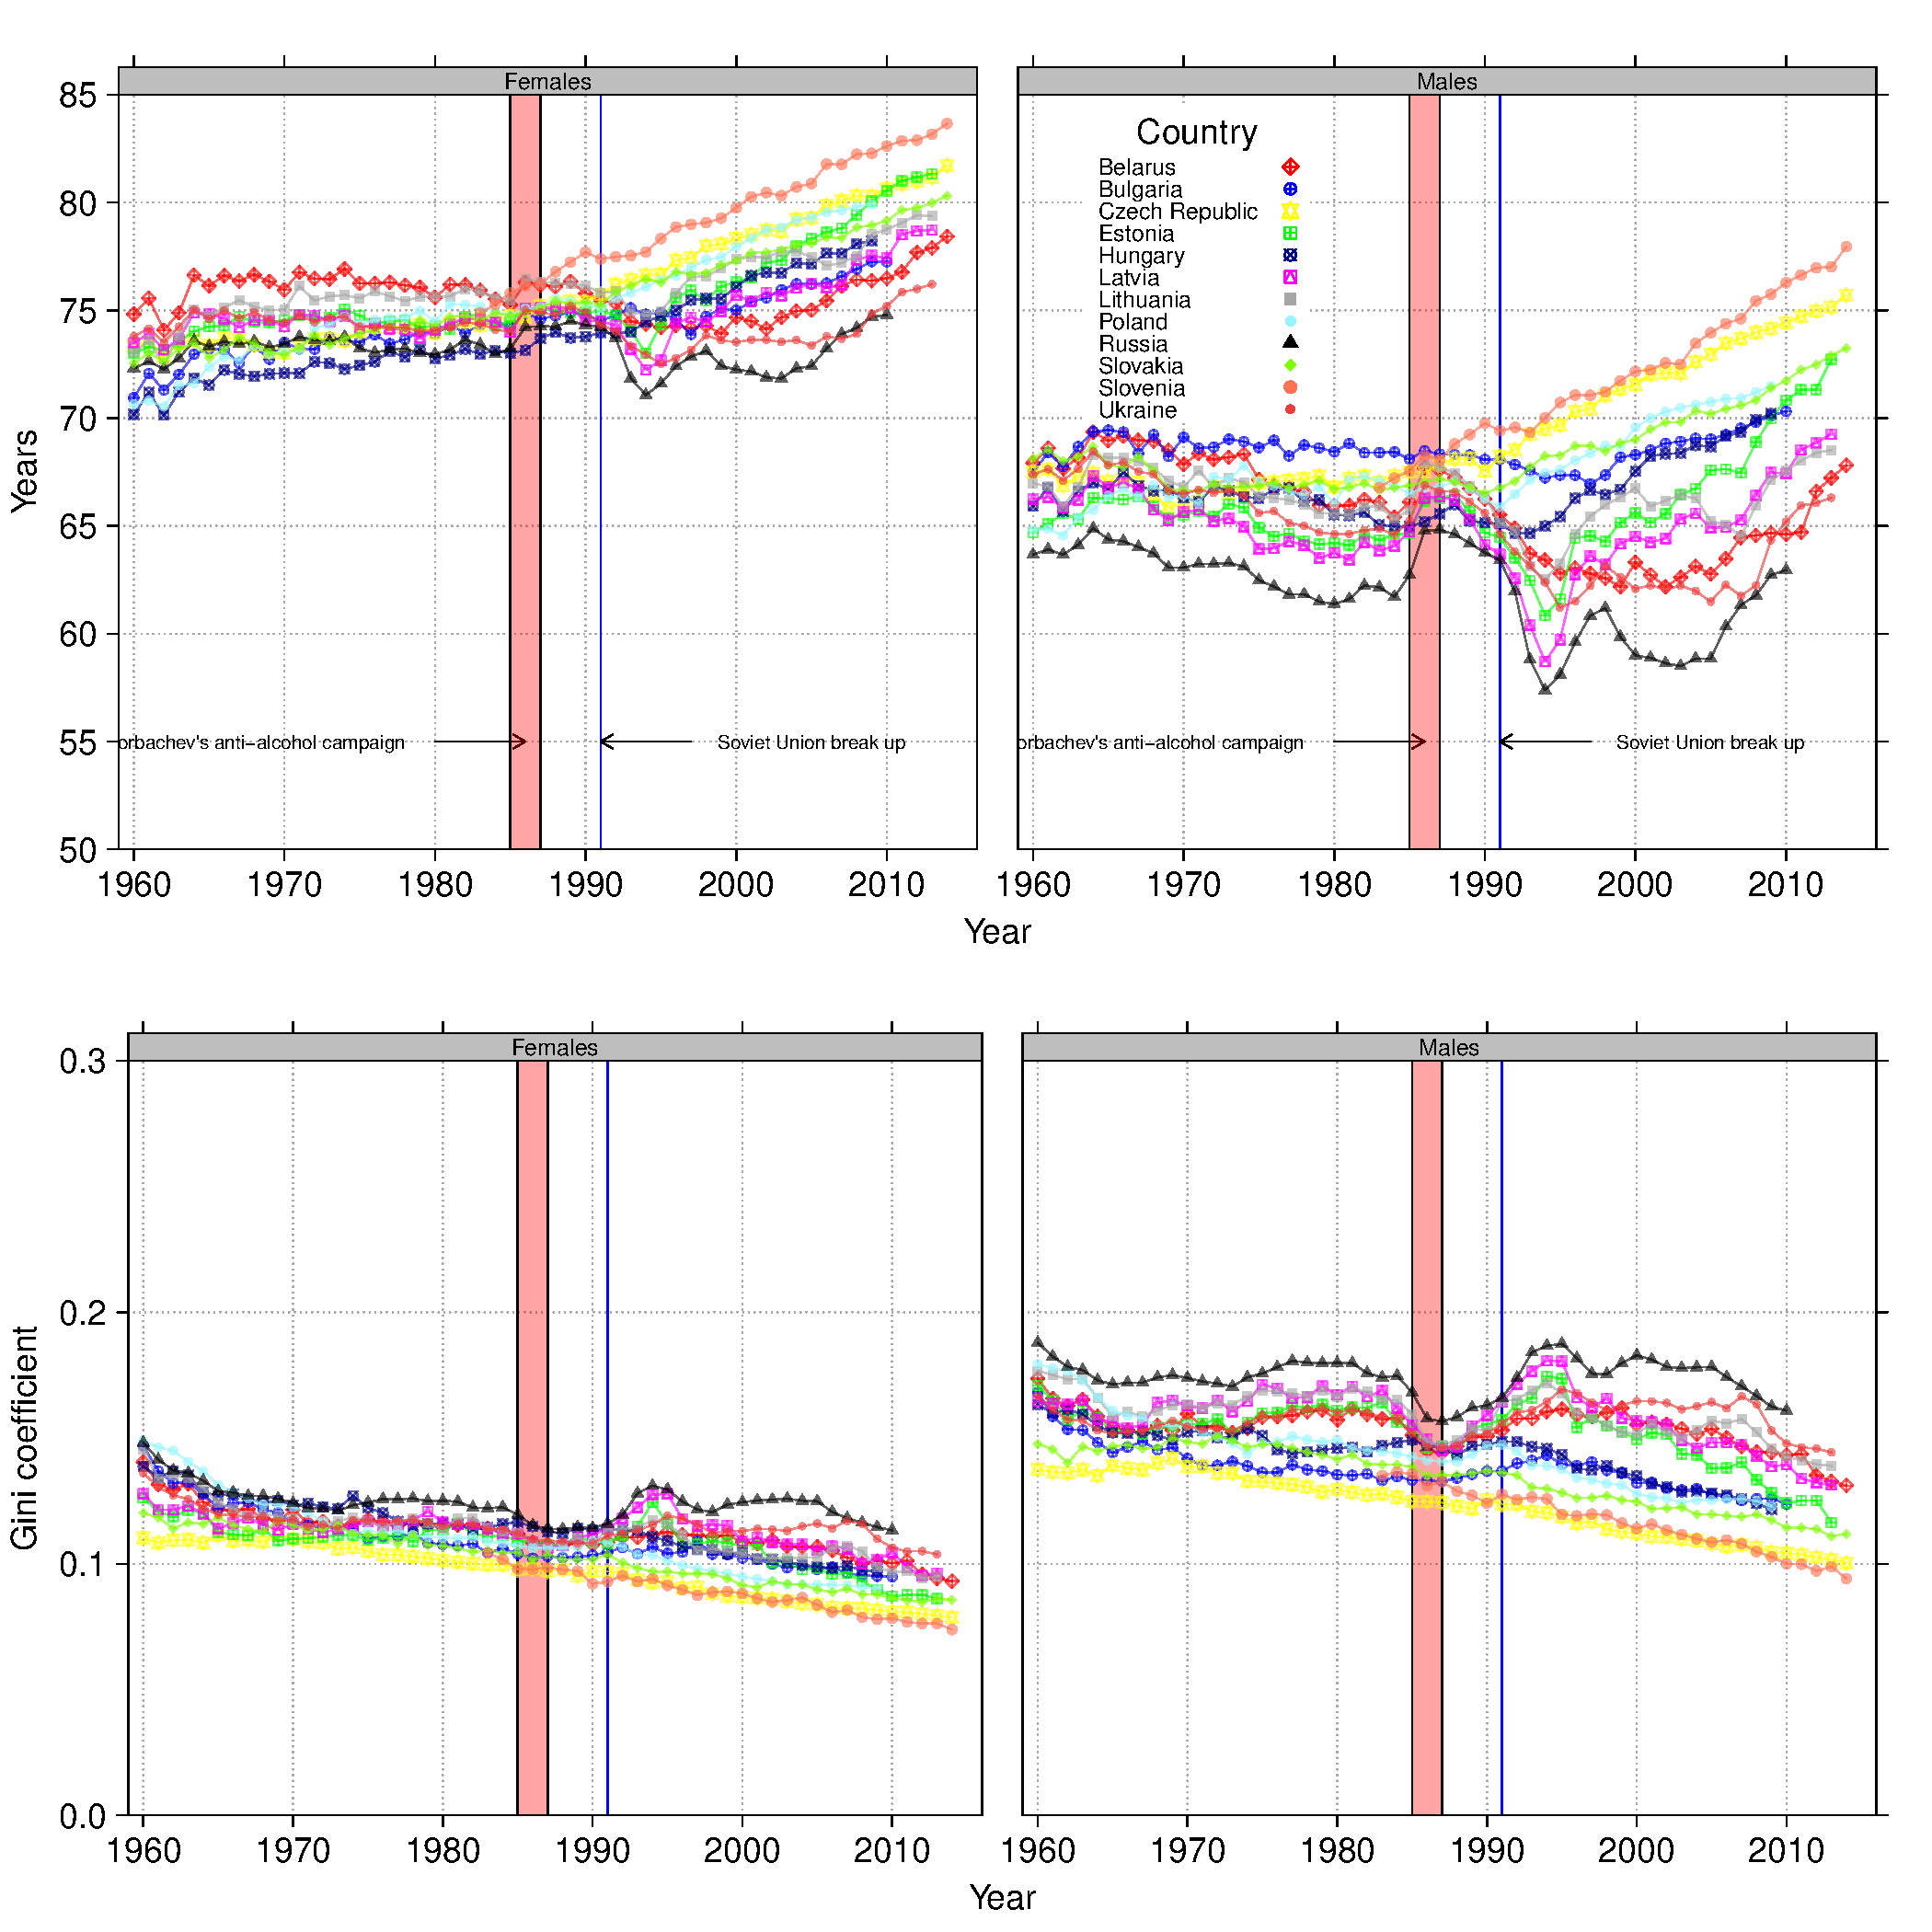
\includegraphics[scale=.4]{Figures/F1_SS}
\end{center}
\end{figure}

\newpage

\begin{figure}[h!]
\caption{Absolute changes in life expectancy and Gini coefficient by sex for Eastern European countries}
\centering
\begin{center}
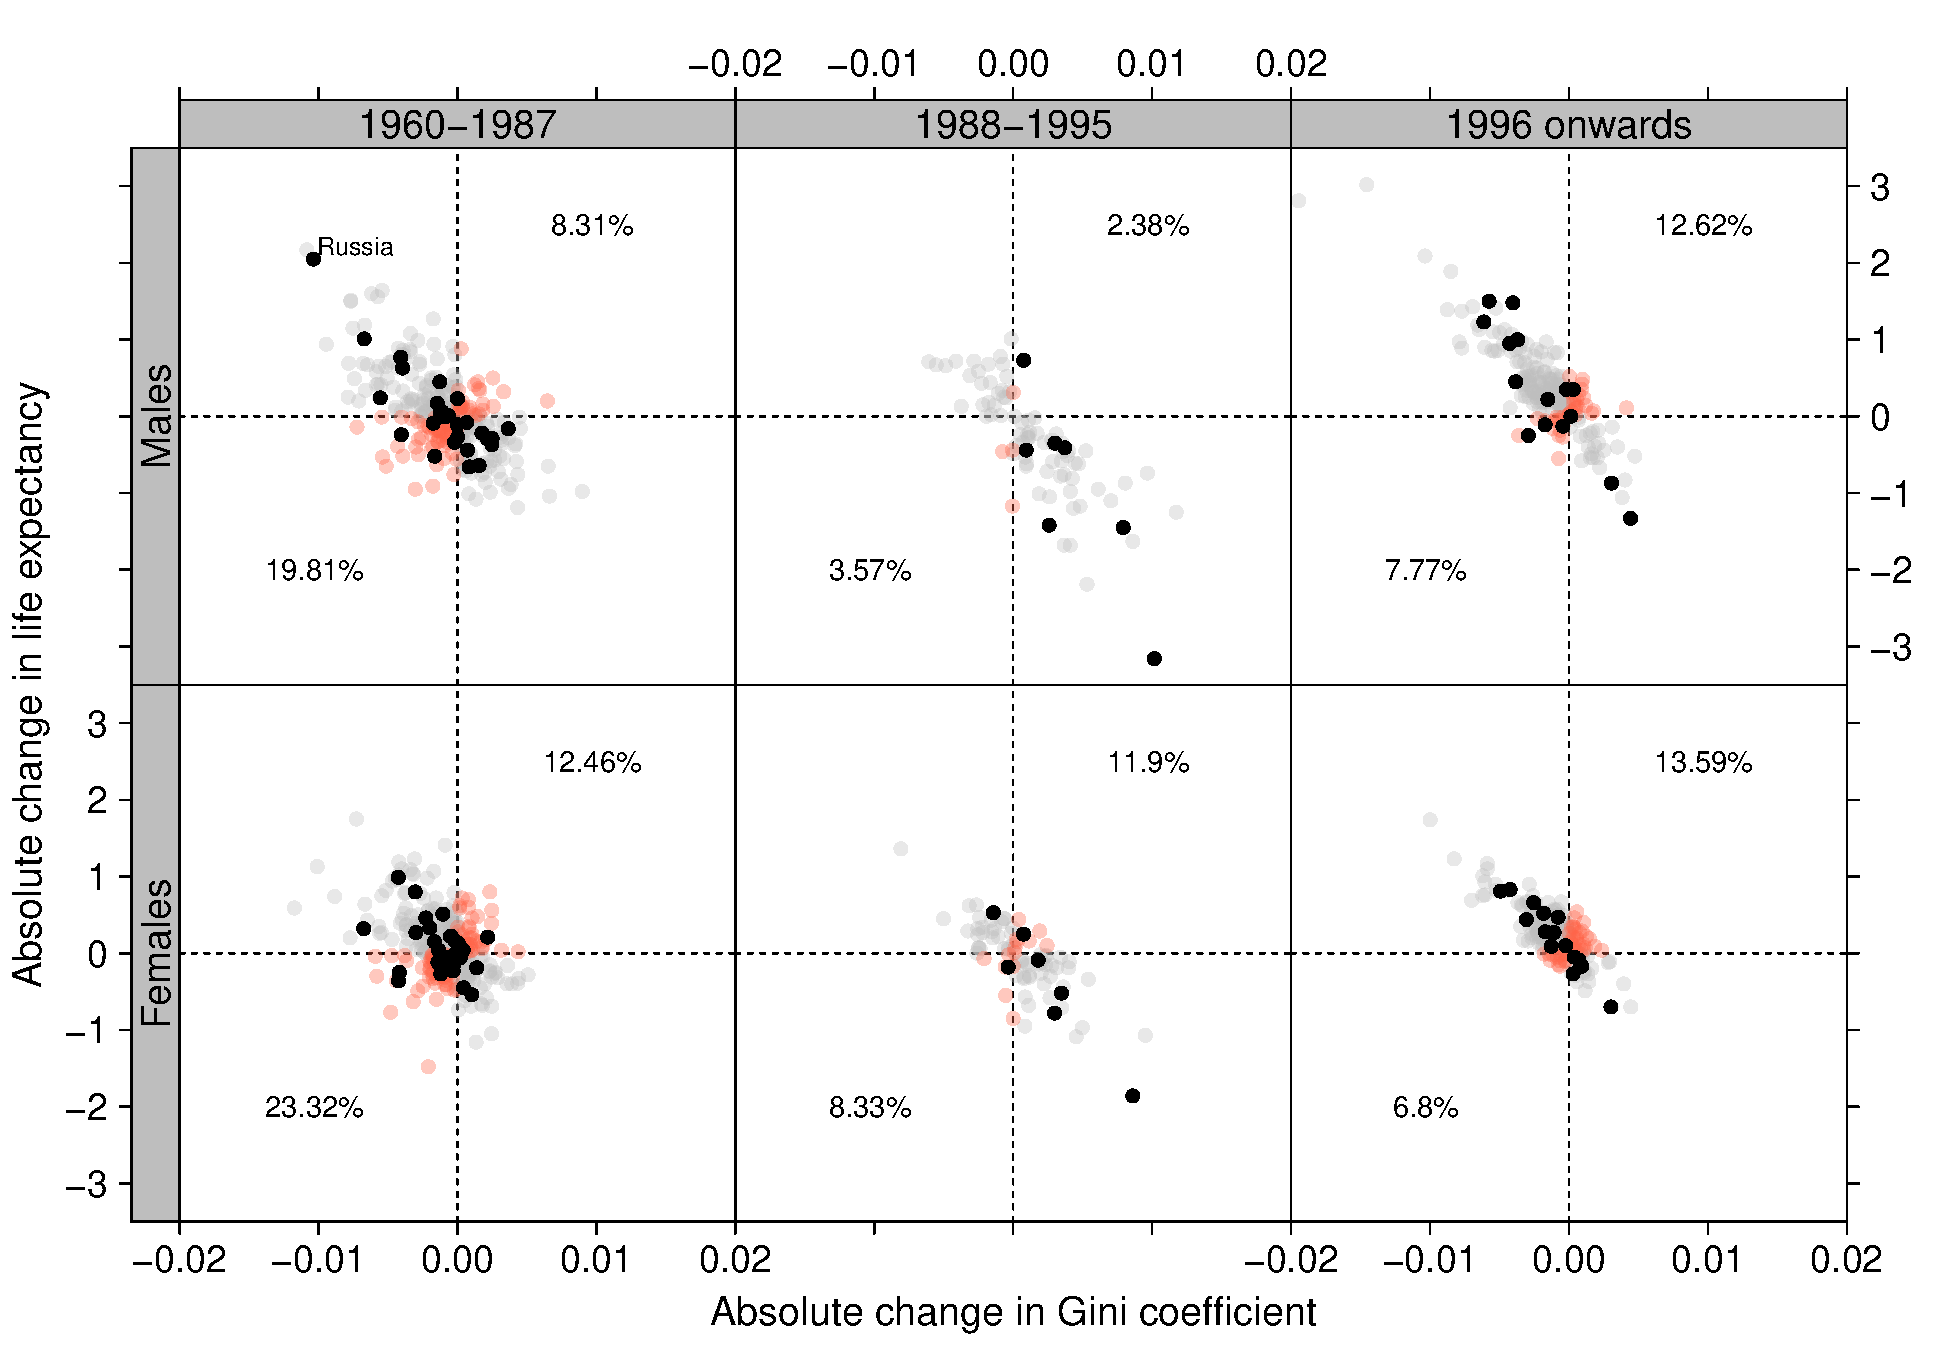
\includegraphics[scale=.4]{Figures/F2_SS}
\end{center}
\end{figure}

\newpage

\begin{figure}[h!]
\caption{Relative changes in life expectancy and Gini coefficient by sex for Eastern European countries}
\centering
\begin{center}
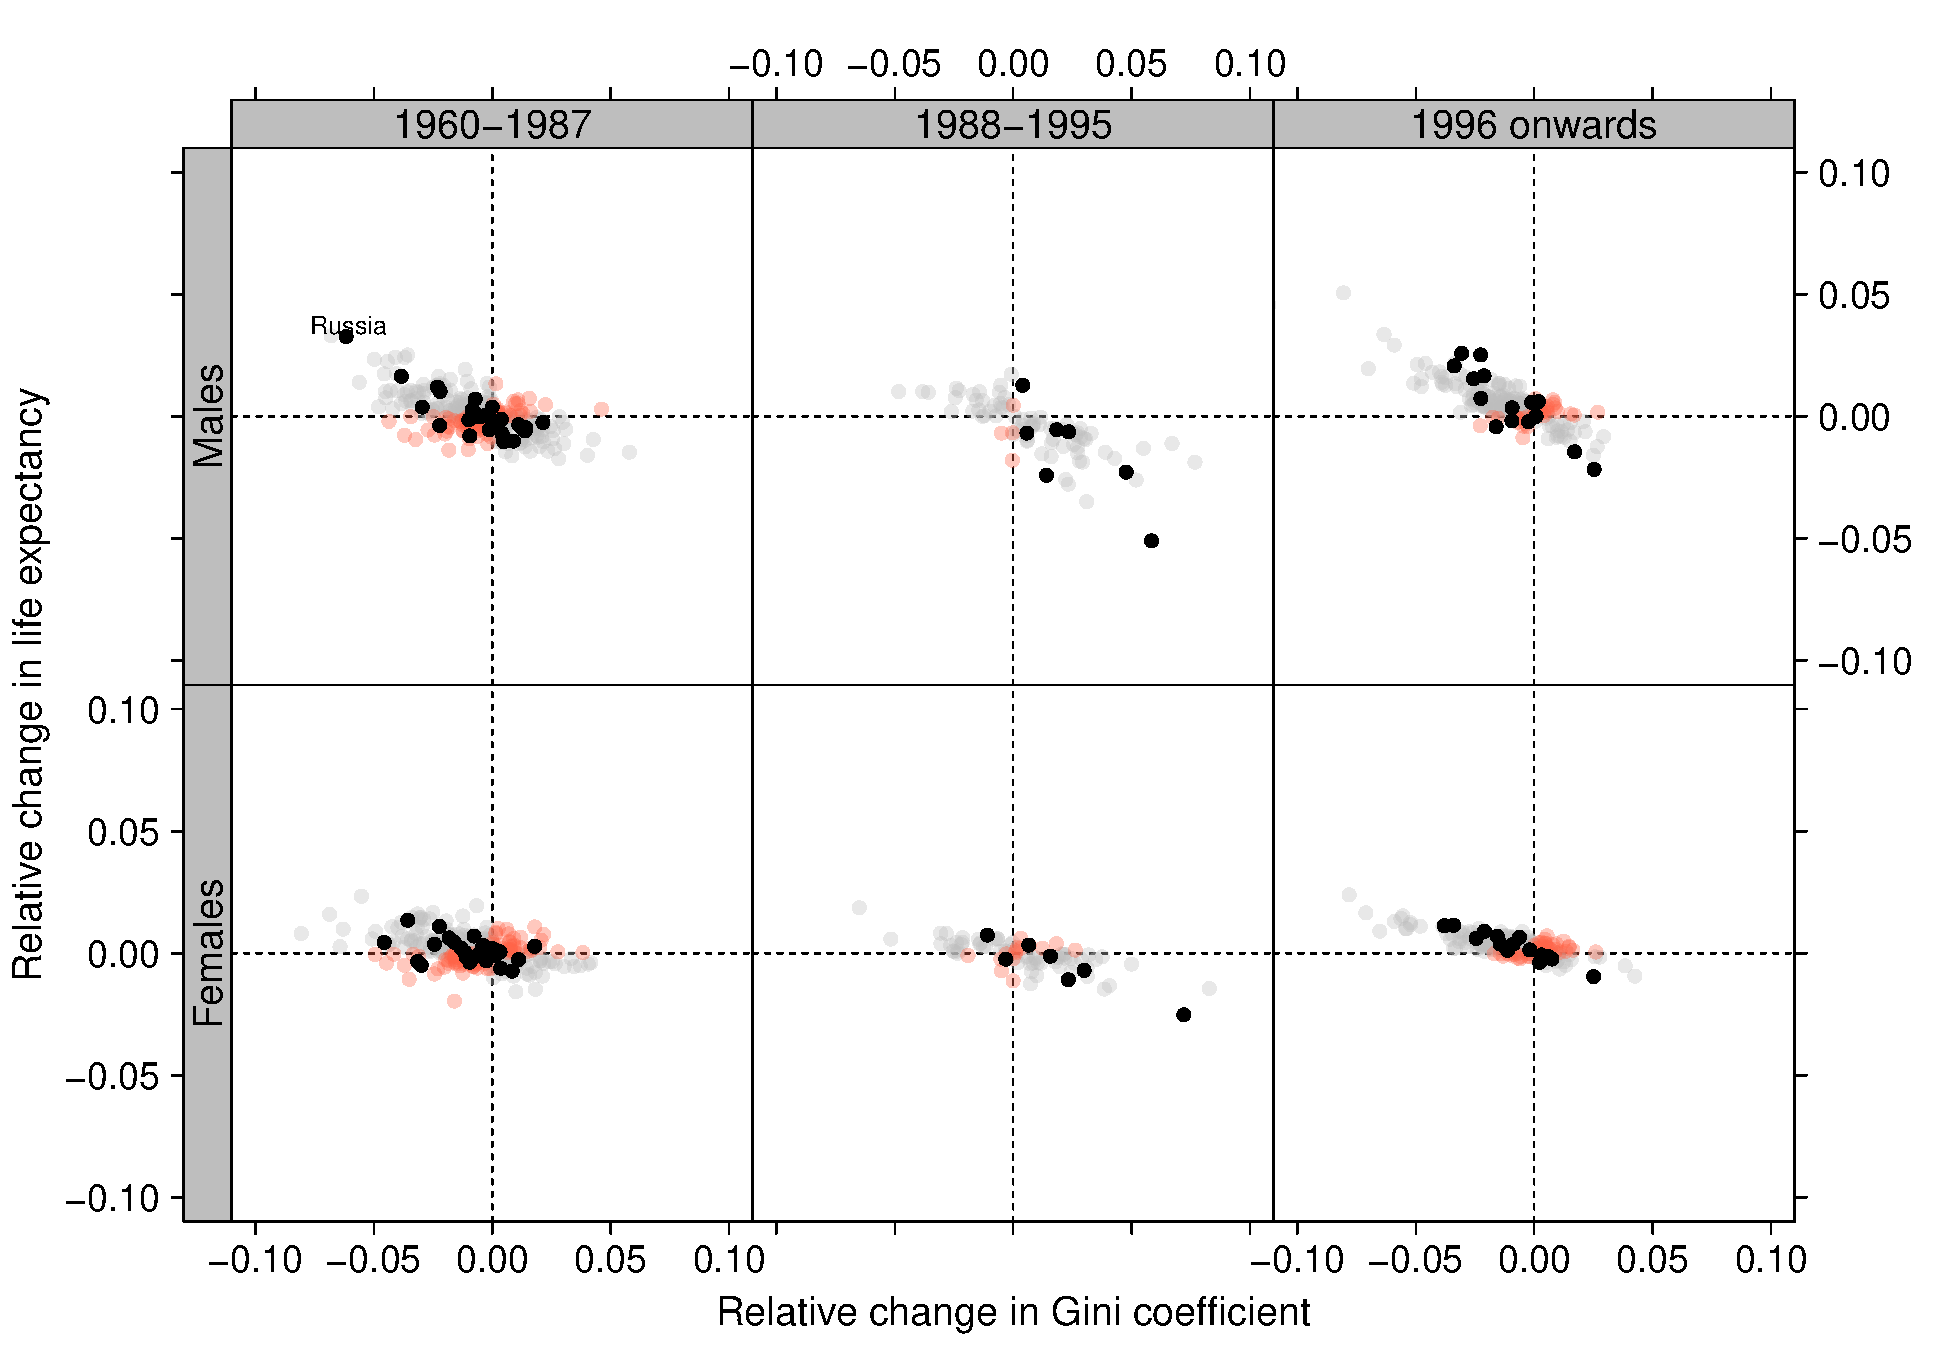
\includegraphics[scale=.4]{Figures/F3_SS}
\end{center}
\end{figure}

\newpage

\begin{figure}[h!]
\caption{Contributions to changes in Gini coefficient by period}
\centering
\begin{center}
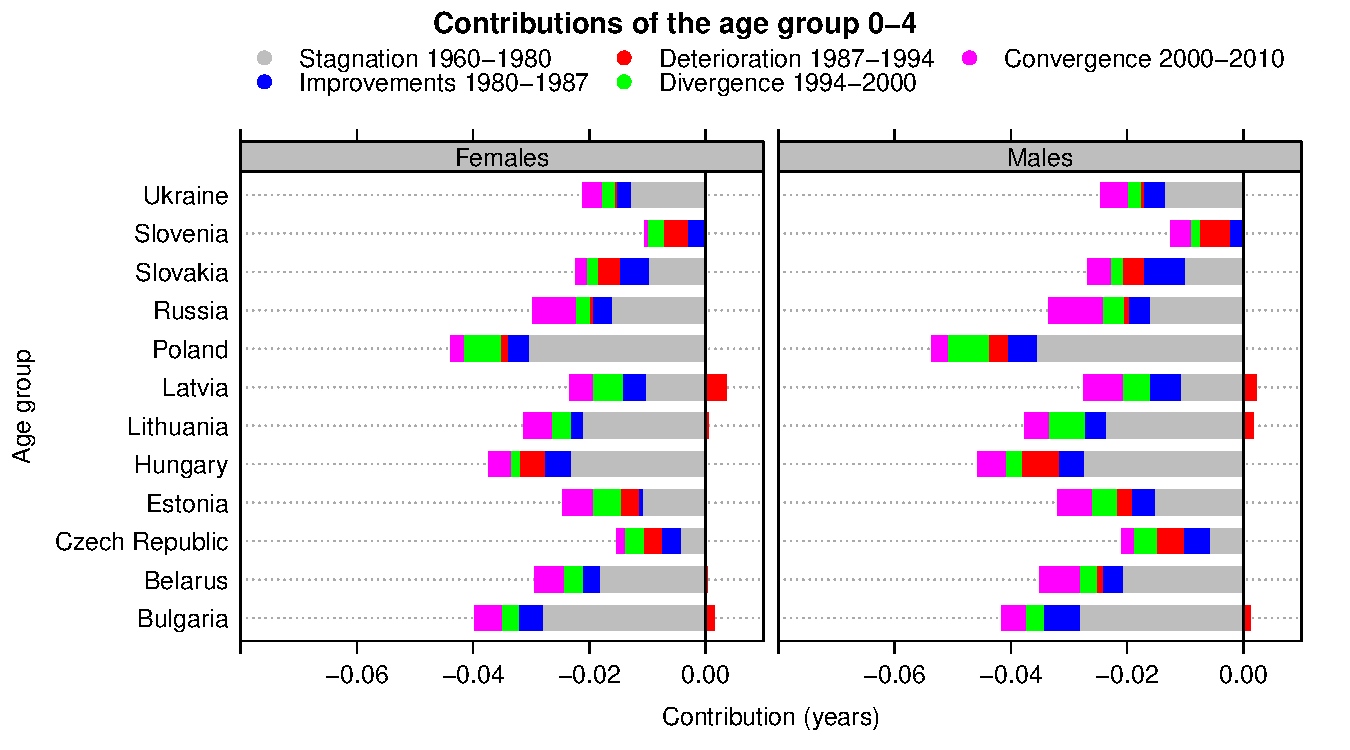
\includegraphics[scale=.6]{Figures/F6_SS_MalesInfant_Periods}
\end{center}
\end{figure}

\newpage

\begin{figure}[h!]
\caption{Contributions to changes in Gini coefficient by period, Males.}
\centering
\begin{center}
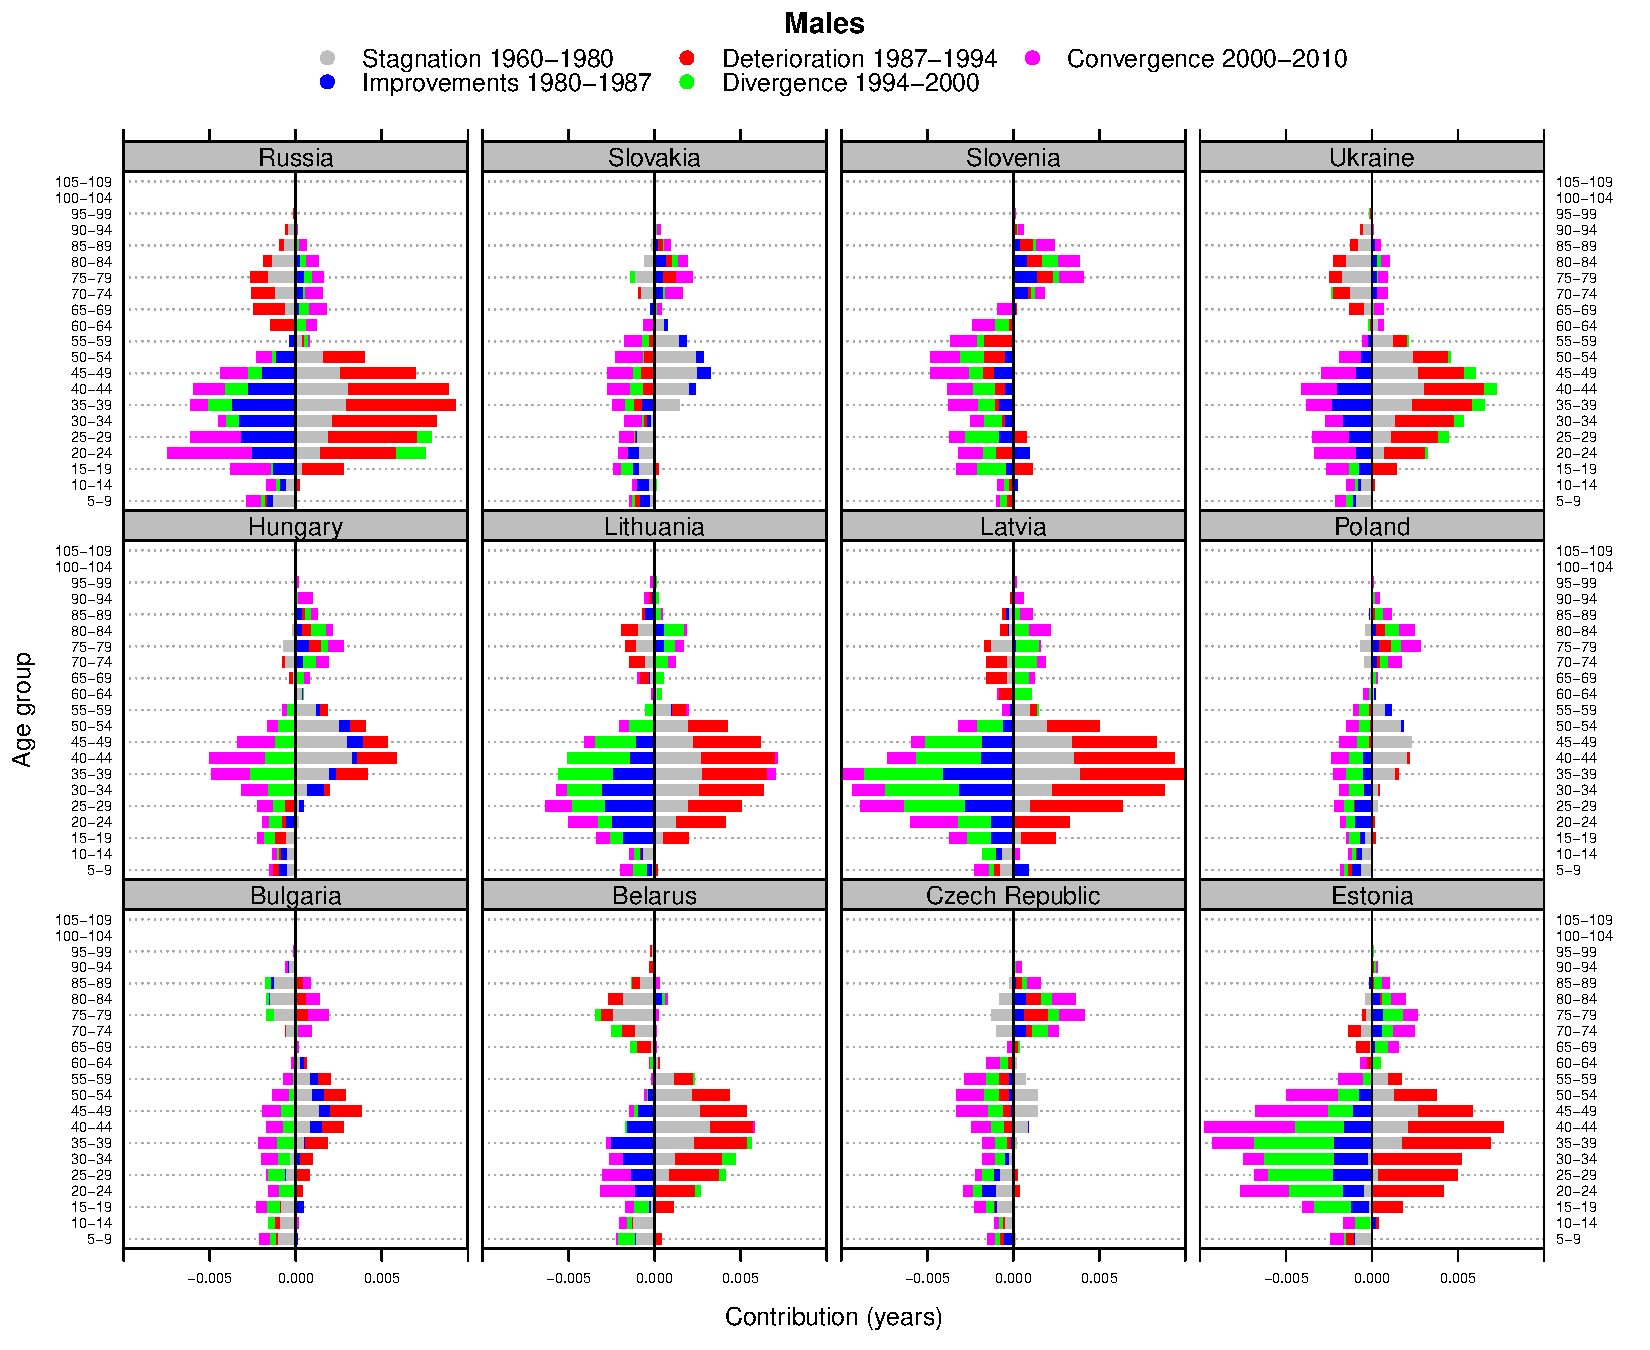
\includegraphics[scale=.54]{Figures/F4_SS_MalesDecomp_Periods}
\end{center}

\end{figure}



\newpage

 \bibliography{Aburto}


%}
%\bibliographystyle{plainnat}


\end{document}
